%%%%%%%%%%%%%%%%%%%%%%%%%%%%%%%%%%%%%%%%%
% Masters/Doctoral Thesis 
% LaTeX Template
% Version 2.5 (27/8/17)
%
% This template was downloaded from:
% http://www.LaTeXTemplates.com
%
% Version 2.x major modifications by:
% Vel (vel@latextemplates.com)
%
% This template is based on a template by:
% Steve Gunn (http://users.ecs.soton.ac.uk/srg/softwaretools/document/templates/)
% Sunil Patel (http://www.sunilpatel.co.uk/thesis-template/)
%
% Template license:
% CC BY-NC-SA 3.0 (http://creativecommons.org/licenses/by-nc-sa/3.0/)
%
%%%%%%%%%%%%%%%%%%%%%%%%%%%%%%%%%%%%%%%%%

%----------------------------------------------------------------------------------------
%	PACKAGES AND OTHER DOCUMENT CONFIGURATIONS
%----------------------------------------------------------------------------------------

\documentclass[
12pt, % The default document font size, options: 10pt, 11pt, 12pt
oneside, % Two side (alternating margins) for binding by default, uncomment to switch to one side
english, % ngerman for German
onehalfspacing, % Single line spacing, alternatives: onehalfspacing or doublespacing
%draft, % Uncomment to enable draft mode (no pictures, no links, overfull hboxes indicated)
%nolistspacing, % If the document is onehalfspacing or doublespacing, uncomment this to set spacing in lists to single
%liststotoc, % Uncomment to add the list of figures/tables/etc to the table of contents
%toctotoc, % Uncomment to add the main table of contents to the table of contents
%parskip, % Uncomment to add space between paragraphs
%nohyperref, % Uncomment to not load the hyperref package
headsepline, % Uncomment to get a line under the header
%chapterinoneline, % Uncomment to place the chapter title next to the number on one line
%consistentlayout, % Uncomment to change the layout of the declaration, abstract and acknowledgements pages to match the default layout
]{MastersDoctoralThesis} % The class file specifying the document structure

\usepackage[utf8]{inputenc} % Required for inputting international characters
\usepackage[T1]{fontenc} % Output font encoding for international characters
\usepackage{pdfpages}
\usepackage{mathpazo} % Use the Palatino font by default
\usepackage{todonotes}
\usepackage{menukeys}
%\usepackage[backend=bibtex,style=authoryear,natbib=true]{biblatex} % Use the bibtex backend with the authoryear citation style (which resembles APA)

%\addbibresource{reference_library.bib} % The filename of the bibliography

\usepackage[autostyle=true]{csquotes} % Required to generate language-dependent quotes in the bibliography

%----------------------------------------------------------------------------------------
%	MARGIN SETTINGS
%----------------------------------------------------------------------------------------

\geometry{
	paper=a4paper, % Change to letterpaper for US letter
	inner=2.5cm, % Inner margin
	outer=3.8cm, % Outer margin
	bindingoffset=.5cm, % Binding offset
	top=1.5cm, % Top margin
	bottom=1.5cm, % Bottom margin
	%showframe, % Uncomment to show how the type block is set on the page
}

%----------------------------------------------------------------------------------------
%	THESIS INFORMATION
%----------------------------------------------------------------------------------------

\thesistitle{Secure PCB Phone Design} % Your thesis title, this is used in the title and abstract, print it elsewhere with \ttitle
\supervisor{Dr. Paul \textsc{Gardner-Stephen}} % Your supervisor's name, this is used in the title page, print it elsewhere with \supname
\examiner{} % Your examiner's name, this is not currently used anywhere in the template, print it elsewhere with \examname
\degree{Bachelor of Engineering (Electronics) (Honours)} % Your degree name, this is used in the title page and abstract, print it elsewhere with \degreename
\author{Lachlan \textsc{McDonald}} % Your name, this is used in the title page and abstract, print it elsewhere with \authorname
\addresses{} % Your address, this is not currently used anywhere in the template, print it elsewhere with \addressname

\subject{Biological Sciences} % Your subject area, this is not currently used anywhere in the template, print it elsewhere with \subjectname
\keywords{} % Keywords for your thesis, this is not currently used anywhere in the template, print it elsewhere with \keywordnames
\university{\href{http://www.flinders.edu.au}{Flinders University}} % Your university's name and URL, this is used in the title page and abstract, print it elsewhere with \univname
\department{\href{https://www.flinders.edu.au/college-science-engineering}{College of Science and Engineering}} % Your department's name and URL, this is used in the title page and abstract, print it elsewhere with \deptname
\group{\href{http://researchgroup.university.com}{Telecommunications Research Laboratory}} % Your research group's name and URL, this is used in the title page, print it elsewhere with \groupname

\AtBeginDocument{
\hypersetup{pdftitle=\ttitle} % Set the PDF's title to your title
\hypersetup{pdfauthor=\authorname} % Set the PDF's author to your name
\hypersetup{pdfkeywords=\keywordnames} % Set the PDF's keywords to your keywords
}

\begin{document}

\frontmatter % Use roman page numbering style (i, ii, iii, iv...) for the pre-content pages

\pagestyle{plain} % Default to the plain heading style until the thesis style is called for the body content

%----------------------------------------------------------------------------------------
%	TITLE PAGE
%----------------------------------------------------------------------------------------

\begin{titlepage}
\begin{center}

\vspace*{.06\textheight}
{\scshape\LARGE \univname\par}\vspace{1.5cm} % University name
\textsc{\Large Honours Thesis}\\[0.5cm] % Thesis type

\HRule \\[0.4cm] % Horizontal line
{\huge \bfseries \ttitle\par}\vspace{0.4cm} % Thesis title
\HRule \\[1.5cm] % Horizontal line
 
\begin{minipage}[t]{0.4\textwidth}
\begin{flushleft} \large
\emph{Author: }\\
\authorname
\end{flushleft}
\end{minipage}
\begin{minipage}[t]{0.4\textwidth}
\begin{flushright} \large
\emph{Supervisor:} \\
\supname
\end{flushright}
\end{minipage}\\[3cm]
 
\vfill

\large \textit{A thesis submitted in fulfilment of the requirements\\ for the degree of \degreename}\\[0.3cm] % University requirement text
\textit{in the}\\[0.4cm]
\groupname\\\deptname\\[2cm] % Research group name and department name
 
\vfill

{\large \today}\\[4cm] % Date
%\includegraphics{Logo} % University/department logo - uncomment to place it
 
\vfill
\end{center}
\end{titlepage}

%----------------------------------------------------------------------------------------
%	DECLARATION PAGE
%----------------------------------------------------------------------------------------

\begin{declaration}
\addchaptertocentry{\authorshipname} % Add the declaration to the table of contents
\noindent I, \authorname, declare that this thesis titled, \enquote{\ttitle} and the work presented in it are my own. I confirm that:

\begin{itemize} 
\item This work was done wholly or mainly while in candidature for a research degree at this University.
\item Where any part of this thesis has previously been submitted for a degree or any other qualification at this University or any other institution, this has been clearly stated.
\item Where I have consulted the published work of others, this is always clearly attributed.
\item Where I have quoted from the work of others, the source is always given. With the exception of such quotations, this thesis is entirely my own work.
\item I have acknowledged all main sources of help.
\item Where the thesis is based on work done by myself jointly with others, I have made clear exactly what was done by others and what I have contributed myself.\\
\end{itemize}
 
\noindent Signed:\\
\rule[0.5em]{25em}{0.5pt} % This prints a line for the signature
 
\noindent Date:\\
\rule[0.5em]{25em}{0.5pt} % This prints a line to write the date
\end{declaration}

\cleardoublepage

%%----------------------------------------------------------------------------------------
%%	QUOTATION PAGE
%%----------------------------------------------------------------------------------------
%
%\vspace*{0.2\textheight}
%
%\noindent\enquote{\itshape Thanks to my solid academic training, today I can write hundreds of words on virtually any topic without possessing a shred of information, which is how I got a good job in journalism.}\bigbreak
%
%\hfill Dave Barry

%----------------------------------------------------------------------------------------
%	ABSTRACT PAGE
%----------------------------------------------------------------------------------------

\begin{abstract}
  \addchaptertocentry{\abstractname} % Add the abstract to the table of contents
  The security of modern smart-phones and computers is impossible to guarantee or to assume due to the out-of-control complexity of
  these devices.  The MEGA65 project seeks to address this by creating simple computing and communications devices that remain
  sufficiently useful in practice. The MEGA65 phone is designed around an open and simple architecture that are simple
  enough to allow highly secure operation.  This requires the ability to isolate, and when necessary de-energise, untrustable
  components like the cellular modem.  This thesis documents the process of developing a schematic and initial printed circuit board
  layout for the MEGA65 phone.  This included elucidation of the functional requirements, selection of hardware components and
  architectural elements that can support those functional requirements, as well development of the circuits to implement each, the
  incorporation of those circuits into a complete schematic design, and the transformation of that schematic design into a printed
  circuit board layout that can be manufactured to form the core of fully functional prototypes of the MEGA65 phone.
  This is made possible in part by targeting a hand-held game-console form-factor, to avoid the need to for extreme miniaturisation,
  which significantly reduces the design effort and cost of manufacturing prototype devices.  Low-cost iteration of the design is
  supported by using a removeable FPGA module, so that the circuit board can be refined without the cost and complexity of purchasing
  and attaching a large BGA part to the main circuit board.  The result is a circuit board that is sufficiently affordable and
  manufacturable to support the future stages of the MEGA65 phone project, without compromising on satisfaction of the functional
  requirements. 
\end{abstract}

%----------------------------------------------------------------------------------------
%	ACKNOWLEDGEMENTS
%----------------------------------------------------------------------------------------

\begin{acknowledgements}
\addchaptertocentry{\acknowledgementname} % Add the acknowledgements to the table of contents
From the completion of this thesis I have gained a lot of wisdom from a number of people in my project team. I would like to thank Hugo Dpr and Tanguy Nodet for their contributions during the year. I would especially like to thank Jayden Grigg and my project supervisor Paul Gardner-Stephen for their contributions and support throughout the entire duration of the project. \ldots
\end{acknowledgements}

%----------------------------------------------------------------------------------------
%	LIST OF CONTENTS/FIGURES/TABLES PAGES
%----------------------------------------------------------------------------------------

\tableofcontents % Prints the main table of contents

\listoffigures % Prints the list of figures

%----------------------------------------------------------------------------------------
%	ABBREVIATIONS
%----------------------------------------------------------------------------------------

\begin{abbreviations}{ll} % Include a list of abbreviations (a table of two columns)

\textbf{CPU} & \textbf{C}omputer \textbf{P}rocessing \textbf{U}nit\\
\textbf{PCB} & \textbf{P}rinted \textbf{C}ircuit \textbf{B}oard\\
\textbf{SD} & \textbf{S}ecure \textbf{D}igital \\
\textbf{SIM} & \textbf{S}ubscriber \textbf{I}dentity \textbf{M}odule\\

\end{abbreviations}

%----------------------------------------------------------------------------------------
%	THESIS CONTENT - CHAPTERS
%----------------------------------------------------------------------------------------

\mainmatter % Begin numeric (1,2,3...) page numbering

\pagestyle{thesis} % Return the page headers back to the "thesis" style

% Include the chapters of the thesis as separate files from the Chapters folder
% Uncomment the lines as you write the chapters

% Chapter Template

\chapter{Introduction} % Main chapter title

\label{Chapter1} % Change X to a consecutive number; for referencing this chapter elsewhere, use \ref{ChapterX}

%----------------------------------------------------------------------------------------
%	SECTION 1
%----------------------------------------------------------------------------------------

This introductory chapter provides an overview of the thesis goals and the basic background behind the method reasoning. The following sections present: (1) the reason for the secure smartphone project; (2) an introduction to the MEGA65 project; (3) the scope, research questions and design requirements of the project. This chapter also provides a brief outline of every section of the thesis. 

\section{The Shared Delusion of Security}

	The last few years has seen a disturbing upward trend in the number and severity of security vulnerabilities in modern computing devices. Whereas traditionally these security vulnerabilities have existed primarily in software, the ever-growing complexity of computer hardware, and in particular CPU designs, now means that we are beginning to see many more hardware-based vulnerabilities.  Whereas software vulnerabilities can be quickly and economically patched, this is not always the case for hardware-based vulnerabilities, as it may require replacement of the defective hardware.  

The recent Spectre and Meltdown vulnerabilities are headline examples of this trend and the difficulties that such vulnerabilities create. Intel and the other vendors are still struggling to produce patches that do not reduce the reliability or performance of their processors, while mitigating as much of the threat posed by these vulnerabilities as possible.  At the end of the day, however, the only fully effective solution is for them to develop a new generation of processors that have the defects corrected in the silicon – an extremely expensive and time-consuming process – and even then, it is likely that the performance of those processors will be impaired, precisely because it is performance optimisations that are the direct cause of the vulnerabilities.  Further, even if we were to assume that corrected hardware were produced, it too could be found to suffer from one or more hitherto unknown vulnerabilities, and it too require replacement.  Put another way, the window of vulnerability for a hardware defect is typically orders of magnitude longer than for a software vulnerability. When commerce, personal privacy and security as well as national security depends on the correct and secure operation of computers, we clearly have a problem of considerable importance before us.

Modern computers are designed to achieve increasing performance and functionality through the easiest route. This is typically done by adding in extra layers of code, consequently increasing sophistication and complicating the system. The processors of these modern computers are optimised using speculative execution, which is a technique used by high-speed processors in order to increase performance by guessing future likely execution paths \cite{RN16}. Unlike older computers, this adds another level of complexity to the computer. This complexity however can be detrimental to security, due to vulnerabilities in the hardware being able to be exploited. There have been a number of recent cases where vulnerabilities have been exploited, in specific the Spectre and Meltdown hardware attacks. 

Spectre attacks involve inducing a victim to speculatively perform operations that would not occur during correct program execution, which consequently leak the victim’s confidential information to the adversary via a side channel \cite{RN16}.  
Meltdown attacks also break the fundamental isolation between the user applications and the operating system. The attack allows a program to access the memory of the affected computer. Which in turn can give away secrets of other programs and the operating system \cite{RN3}. 


%-----------------------------------
% 	SECTION 2
%-----------------------------------
\section{The MEGA65 Project}

	The overall project aim is to create a secure smartphone based on a purposely simple architecture, that is capable of basic telephony functions and simple productivity tasks. Where a trade-off must be made between security and richness of functions, the trade-offs will tend to the secure side. The sufficiently functional system’s architecture will be based on the Commodore 64 computer, to ensure that the device is secure as well as allowing its existing productivity software, tools and developer base and knowledge to be leveraged. 
	The MEGA65 project was created to develop the unreleased Commodore 65 (C65). Collaborators from all around the world build pieces of the puzzle. The recreated system is 50 times faster than the original Commodore 64 and is an exact replica of the original C65. The C65 operating system would provide a sufficient foundation for a secure mobile device, due to its simplistic architecture.  
	This report will focus on the development of the PCB which will hold the circuitry for the smartphone. 


%-----------------------------------
%	SECTION 3
%-----------------------------------

\section{Research Questions \& Scope}
The following questions were derived to help build a foundation for the research:
\begin{enumerate}
\item What power control circuitry can satisfy the security-driven requirement of the MEGA65 to be able to power down all communications hardware when required, yet remain able to be woken by that same hardware?
\item What trade-offs, if any, are required to satisfy the functional and dimensional requirements of the MEGA65 phone PCB?
\end{enumerate}

\subsection{Design Requirements}

To design a secure phone with the intentions of it being untraceable if need be, it’s underlying architecture would need to be as simplistic as possible. To ensure that the phone can remain secure at all times the following design requirements are required:
\begin{itemize}
\item Whilst the device is in secure mode, any component which can remain stable between power cycles must be disabled, so that there is no easy mechanism for the exfiltration of data from the device. This includes turning off the untrusted mobile phone modem. 
\item Only need FPGA to be powered up when needed to, so the 4G modem is required to be able to wake the FPGA if the modem is on.
\item The FPGA needs to be able to turn off the phone radio, when it wants to.
\item Physical manual override power switches are required that will allow the user to power down the modem. This will effectively be an Air-plane mode feature. 
\end{itemize}
The modem also has a high-power consumption (approximately four amperes) that needs to be electronically switched. These objectives require research into different circuit options, including power control circuitry; and state diagrams for the transitions.

%-----------------------------------
%	SECTION 4
%-----------------------------------
\section{Structure of Thesis}

Following this chapter, Chapter \ref{Chapter2} provides background information on the project, including an in depth study on the insecurity of modern complex CPUs.\\ Chapter \ref{Chapter3} follows this with a list of required use cases of the secure phone with a list of functional requirements based on the needs of the use cases.\\ 
In Chapter \ref{Chapter4} a list of hardware requirements is made from the list of functional requirements.\\
First, Chapter \ref{Chapter5} begins by giving an overview of all the schematics designed from the hardware requirements. Section 2 details the component selection and the method behind this. Section 3 gives detail of the errors in the schematic designs and how they were solved. Section 4 describes the testing phase of the project.\\
Chapter \ref{Chapter6} describes the derivation of the PCB layout from the schematics. This chapter starts by giving details about the footprint design and the method behind them, with the second section going over the PCB layout and template of the phone, with the third section detailing the challenges found throughout the process.\\
Chapter \ref{Chapter7} provides the results and discussion section of the project.\\
Finally, the conclusion of the project is provided in Chapter 8. This summarises the project's goals and results, draws conclusions, and closes the dissertation with suggestions for further research.

% Chapter Template

\chapter{Literature Review} % Main chapter title

\label{Chapter2} % Change X to a consecutive number; for referencing this chapter elsewhere, use \ref{ChapterX}

This chapter provides background information on the reasoning behind the secure phone project. This consists of: (1) an introduction into the state of complex modern processors; (2) a brief history of computer processors; (3) a study into the verification of CPUs, which includes a graph detailing the large rise in the number of transistors per employee per new processor released; (4) security vulnerabilities, which looks at cases where vulnerabilities have been found or are imminent; (5) secure phones, which looks at the history of past secure devices and technologies; (6) a brief overview of the MEGA 65 project; (7) a description of the design software used for the project.\\

%----------------------------------------------------------------------------------------
%	SECTION 1
%----------------------------------------------------------------------------------------

\section{Literature Review}

Since the beginning of modern pipelined microprocessors, computers have become increasingly complex. This complexity can bring about vulnerabilities deep within the software and hardware of a computer. Vulnerabilities are often found through dedicated research and analysis of the specific operating system or component, with the solution to the problem often taking a significant amount of time to find. In some cases, it isn’t certain that a solution can be found without drastically altering the computer hardware or software. 
Smartphones have grown exponentially in terms of their development and their capabilities over the past decade. This growth has led to a more complex processing unit and interface, which in turn, has brought about similar security concerns to ones that can be found within a computer \cite{RN27}. The Apple A11 chip for example, used in the iPhone X, has a staggering four billion transistors \cite{RN28}, which is comparable to many high-end processors currently being released. With the emphasis of smartphones being on functionality, and with brands using increased functionality as a major selling point, the security of these devices has suffered. More functionality brings with it increased complexity, which leads to increased attack surfaces, culminating in increased volumes of vulnerabilities, as already seen in modern computers.
This literature review explores this space, summarising a brief history of CPUs, how CPUs are verified, security concerns, and previous research into secure phones as a prerequisite to considering how smartphones with radically improved security properties can be created.

%----------------------------------------------------------------------------------------
%	SECTION 2
%----------------------------------------------------------------------------------------

\section{A Brief History of Computer Processors}

To begin delving into the complexity of modern processors, a look back into the history of computer processors can provide reasoning for the secure smartphone project. 
In 1968, the Intel Corporation was founded by Robert Noyce and Gordon Moore \cite{RN2}. Eight years prior to this, IBM became the first company to automatically mass-produce transistors \cite{RN2}, with Moore becoming the namesake of Moore’s Law. By 1971 the first microprocessor was introduced, the Intel 4004. The Intel 4004 microprocessor was produced on two-inch wafers, compared to twelve-inch wafers used in present microprocessors, consisted of 2,300 transistors, and was unique in being the smallest microprocessor design that ever went into production \cite{RN5}.

\begin{figure}
	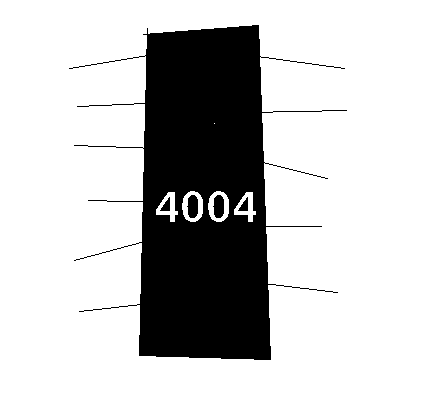
\includegraphics[width=\linewidth]{4004.jpg}
	\caption{Intel 4004 processor \cite{RN9}}
	\label{fig:4004}
\end{figure}

MOS Technology released the 6502 processor in 1975, with it consisting of 3,510 transistors. At the time, the processor sold for less than one-sixth of the price of competing processors from larger companies \cite{RN29}. The 6502 or its variations were used in popular home video game consoles such as the Atari 2600, Apple II, Nintendo Entertainment System and the Commodore 64. Commodore International purchased MOS Technology outright soon after the 6502’s release \cite{RN29}.
The Intel 8080, consisting of 4,500 transistors, was released in April of 1974 and was a significant improvement over the Intel 4004 \cite{RN8}. The 8-bit parallel central processing unit (CPU) was fabricated on a single LSI (Large Scale Integration) chip and used Intel’s n-channel silicon gate MOD process \cite{RN10}. The successors to the 8080, in particular the 8086 – released in 1976 and the 8088 – released in 1979, were fundamental in the development of the modern, complex CPU. The 8086 and 8088 incorporated a significant increase in transistors over their predecessor with each containing 29,000. Many computers today still contain fundamental aspects of the 8086 chip \cite{RN11}.  
When the Motorola 68000 was released in 1980 it was one of the most powerful chips on the market \cite{RN18}. With 68,000 transistors the chip was predominately used in the Apple Macintosh, Sun UNIX work stations, the Commodore Amiga line of computers, printers and video game consoles \cite{RN18}. 
In early 1993 Intel introduced the Pentium processor. With 3.1 million transistors  (Intel, N/A) the processor was the first to incorporate Intel’s super-scalar design. Intel made large sacrifices of performance, power consumption and cost for the sake of maintaining the compatibility with legacy x86 code \cite{RN13}. Intel estimated that 30\% of the Pentium’s transistors were used solely for providing x86 legacy support \cite{RN7}. For this reason the processor lagged behind it’s RISC competitors in performance, while being more complex in its design.
In June of 1998 the Pentium II Xeon 400 processor was released, with it being the first Xeon processor. The processor was the first Intel processor to be packaged in a cartridge, hosting a PCB with the CPU core as well as two or four L2 cache chips \cite{RN12} and consisted of 7.5 million transistors \cite{RN19}. Intel’s plan was to have the Xeon provide a workstation performance at a lower price, while being able to run x86 workstation software on the same system as the normal office software \cite{RN12}.
Much later on in 2006 Intel released the Core 2 Duo processor, a significant improvement over the Pentium processors. The processors started out with over 200 million transistors. 
This lead to the start of the Core i3, i5 and i7 processors with the first generation being released in 2008 with the 8th generation being current. The first i7 processors in 2008 started out having around 731 million transistors and as of today there as processors eclipsing 5 billion.  
	As computers have become both faster and more powerful in all levels of execution they have consequently become far more complex and problematic to debug. The latest Intel processor errata documents are longer than the entire operation manuals for their first processors ever made. The errata of modern processors is more complex than the entire definition of early CPUs.

%----------------------------------------------------------------------------------------
%	SECTION 3
%----------------------------------------------------------------------------------------

\section{Verification of CPUs / Formal Analysis}

	One of the major issues manufacturers of modern computers face is functional verification. In 2001 ARM released that their method of verifying their CPUs, so that the highest possible verification coverage could be achieved, was a process called ‘deterministic simulation’ \cite{RN6}. This was a common and well understood methodology where test cases would be created to be used as self-checking assembler sequences. These cases would then be re-run on a simulation test bench consisting of an ARM CPU, a simple memory model and some simple memory-mapped peripherals. The tests would then be classified into two categories. Although these tests singled out most errors within the CPU, full coverage of the system was not possible with this methodology.
Figure \ref{fig:transistor_graph} shows the number of transistors in a CPU divided by the number of employees at Intel against the processors of the given year. Transistor count is a proxy for the complexity of a chip design, and employee count is a proxy for the amount of design verification effort that the company is able to apply. That is, the graph approximates the complexity to verification effort ratio at Intel over several decades. Higher values are worse, corresponding to reduced scrutiny of the design on a per-transistor basis. While this measure is imperfect in a number of ways, including that Intel’s verification workforce may vary as a fraction of total work-force, and that it is expected that significant productivity increases are likely over the time period, for example through the creation of improved automated verification tools, it is obvious that this measure has increased by around five orders of magnitude over the 45 or so years covered. While the data are not inclusive of every model of processor produced by Intel, it does also show a simultaneous trend to release more processors per unit time, thus spending the verification effort more thinly, even allowing that many contemporary models of processor will have large parts in common. 
	Circumstantial evidence of the difficulty of verifying modern complex processor designs, and that verification effort is being increasingly thinly spread, comes from the recent discovery of the Meltdown and Spectre attacks. These attacks affect processors first produced a decade or more ago, as shown in Figure \ref{fig:transistor_graph}. In the intervening time Intel, AMD and other makers of affected processors have produced many successive generations of processors, apparently without discovering these vulnerabilities. The alternative hypothesis is that they did in fact know about it, and concealed this information. If this were the case, then it would represent a very concerning situation, and would be an even stronger argument for the need for independently verifiable processor designs. Many of the problems found within the hardware can require a full re-design of the processor to eliminate.

\begin{figure}
	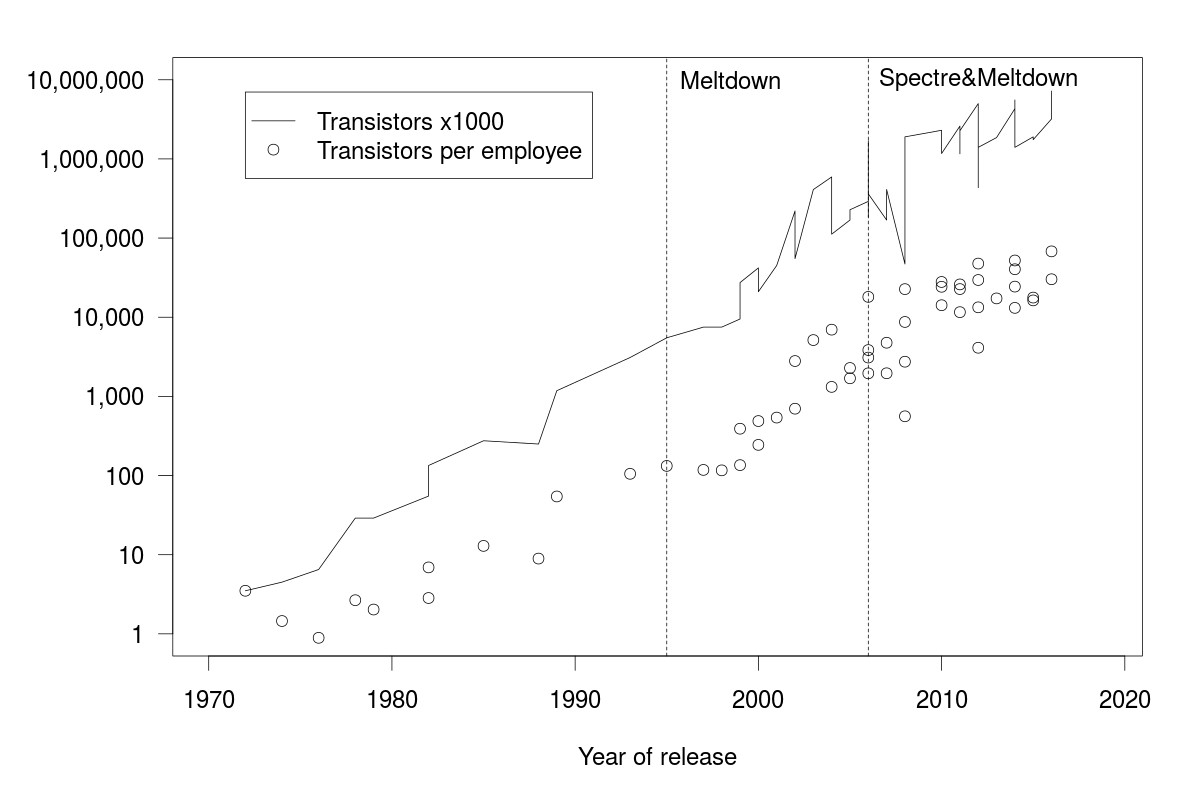
\includegraphics[width=\linewidth]{graph.jpg}
	\caption{Transistors per number of employees at Intel against the number of transistors in their processors that year \cite{RN22, RN23, RN24, RN25, RN26}}
	\label{fig:transistor_graph}
\end{figure}

%----------------------------------------------------------------------------------------
%	SECTION 4
%----------------------------------------------------------------------------------------

\section{Security Vulnerabilities}

	In parallel with the rise of the number of transistors in a CPU there has also been a rise in the number of vulnerabilities and areas in which the CPU can be manipulated. The number of reported software and hardware vulnerabilities grows constantly, with an approximate doubling rate beginning in 2017 \cite{RN17}. The Spectre and Meltdown attacks (as previously mentioned) affect both the hardware and software of nearly every CPU from the past twenty years \cite{RN15}. Spectre attacks involve causing a victim processor to speculatively perform operations that would not occur during correct program execution. This can lead to the victim’s personal and confidential information being leaked via a side channel to the adversary \cite{RN16}. Meltdown attacks predominately involve the hardware of a CPU, in particular the speculative execution features that allow a processor to reduce the time cost of branch instructions, by guessing whether the branch will be taken, and rolling back only if the guess was incorrect. In particular, they rely on the fact that roll-back is not perfect, and that changes to cache occupancy changes can be detected post mortem, that can be used to deduce the contents of arbitrary memory locations to which the program has no permission to access \cite{RN3}.


%-----------------------------------
%	SUBSECTION 1
%-----------------------------------

\subsection{National Security Risks}

	Effectively the same high-level security concern was raised in March of this year concerning the 5G network. The Australian Government are aware that Huawei, a respected smartphone manufacturer in China, are intending to bring their 5G technology to Australia, which could potentially introduce new threats and vulnerabilities. After having already been blocked from tendering for the National Broadband Network in 2012, 5G could potentially be an alternative to the NBN as well, which could potentially persuade customer’s preferences due to it having a faster mobile network. 
	The government’s concern is that Huawei’s technology could lead to security concerns down the track if there is a war between countries and Australia suddenly becomes a hostile adversary. If Huawei were able to go ahead with their plan, eventually all mobile devices will be connected to the 5G network. This would leave all 5G mobiles vulnerable to potential attacks, with the trust of security being left in the phone provider’s and network carrier’s hands. The problem is not that any vulnerability in Huawei equipment has been identified, or even that there has been any proven intention to miss-use the technology in this way. Rather, the problem is simply that the government is unable to be sure that this is not the case, and that uncertainty stems directly from the impossibility of fully verifying he hardware and software components of such complex systems. Therefore, the government has had to assume that the possibility is a real risk to national society.
However, if the user was able to manually turn off the phone’s connection to this network, the threat of a potential attack would be mitigated \cite{RN14}.

%----------------------------------------------------------------------------------------
%	SECTION 5
%----------------------------------------------------------------------------------------

\section{Secure Phones}

	In the past there have been many attempts at creating a secure mobile device, however many have been unsuccessful in being able to fully remove any of the major vulnerabilities due to them still being based on complex CPUs and operating systems. 
	An attempt to encrypt telecommunications occurred in the 1920s. The encrypting device combined a “noise” signal with the audio message, effectively scrambling it, before transmission. The receiver device who would know how to duplicate the “noise signal, would remove the noise to retrieve the original message \cite{RN30}.
	SIGSALY was developed in 1941 as a digital speech encryption system. The system used the unbreakable One-Time Pad encryption scheme, and was used heavily in World War II for confidential conversations between British Prime Minister Winston Churchill and United States President Franklin Roosevelt \cite{RN21}. Although highly secure the One-Time Pad encryption scheme was expensive and in 1943, only 12 SIGSALY terminals were set up around the world \cite{RN21}.

\begin{figure}
	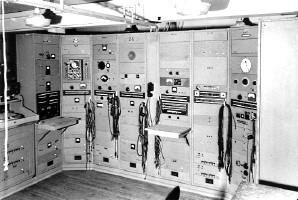
\includegraphics[width=\linewidth]{terminal.jpg}
	\caption{The transmitting side of a SIGSALY terminal /cite{RN21}}
	\label{fig:SIGSALY}
\end{figure}

	The STU-I phone, a secure desk telephone used by the Government of the United States of America and its contractors, arrived in 1970. It had a successor, the STU-II, and replaced the STU-I in 1975. The third iteration, the STU-III was introduced in 1977, with it being on the first applications of asymmetric cryptography \cite{RN30}. Today the United States Government still use STU phones for secure government telecommunications \cite{RN30}.
	In terms of mobile phones, Blackberry sell themselves on producing secure phones. When booted up, their smartphone’s system check both the hardware and software components on the device to ensure that nothing has been tampered with. Full-disk encryption is also offered on the phones to protect private information as well as the choice for a numeric, alphanumeric or picture password. The devices however are still based around a modern complex CPU and hence still have underlying vulnerabilities, for example in 2017 where Blackberry had to notify it’s users about the impact of “BlueBorne” \cite{RN20}, a collection of issues with the implementation of Bluetooth on a variety of software platforms. 
	It can be seen from the past that as the CPU in smartphones becomes more complex the ability to be able to secure it effectively decreases. 

%----------------------------------------------------------------------------------------
%	SECTION 6
%----------------------------------------------------------------------------------------

\section{MEGA 65 Project}

	The MEGA 65 Project is a joint venture of the Resilient Telecommunications Laboratory at Flinders University and the German based MEGA team and a number of volunteer contributors to bring to life the Commodore 65, the unreleased improvement over the Commodore 64 computer. The MEGA 65 CPU is an enhanced 4502 8-bit processor, non-pipelined with no branch-prediction and no cache. The operating system runs in one hypervisor and includes inter-process communication. The following table displays the specifications of the MEGA 65. 



	The project to create a secure smartphone device is in cooperation with the MEGA team and has the aims of recreating the original 8-bit computer to its original specifications, with some improvements including replacing the floppy disk drive with an microSD card drive. The project involves designing both the hardware and software for the secure phone. 

\begin{figure}
	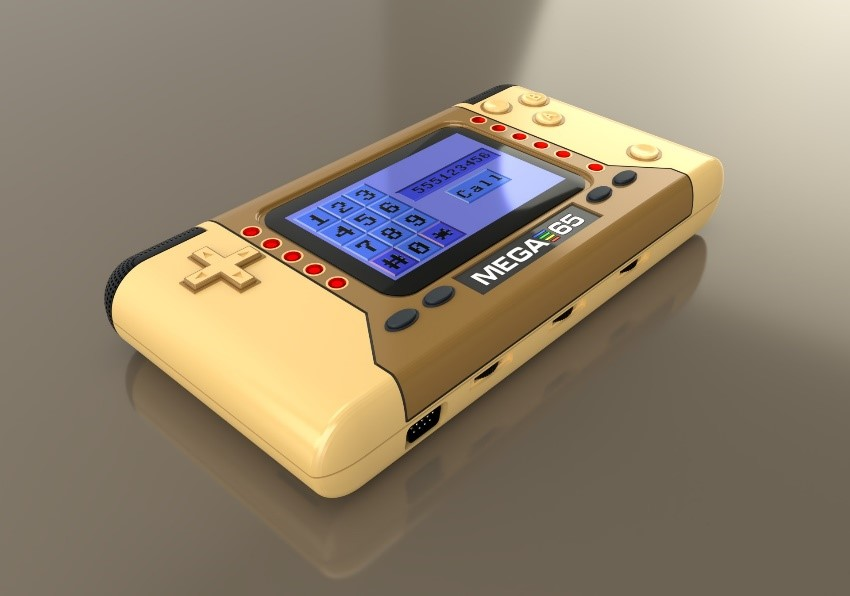
\includegraphics[width=\linewidth]{render.jpg}
	\caption{MEGAPhone Prototype Render}
	\label{fig:render}
\end{figure}

	The secure device will have the capability to be able to disconnect from the world by having a mechanical switch to power its modem on and off, as well as having an advanced encryption system and multiple SIM card slots. The phone will be designed for security over functionality, in contrast to many modern smartphones. All design choices including the routing stage of the PCB will be completed with security in mind, with an FPGA board being used as the CPU.
	One of the major challenges in making the device fully secure, is ensuring that the modem can be turned on and off, when desired without directly affecting the state of the other components. 
	Research is needed in this topic due to the increasing risks in computer security, and the lack of secure mobile devices, considering the age in which we live in where everyone’s personal details are linked to their smartphones.

%----------------------------------------------------------------------------------------
%	SECTION 7
%----------------------------------------------------------------------------------------

\section{Design Software}

	Altium Designer is a software-based schematic and PCB design program. The software has the ability to create complex designs, of any nature – accurately. There are also a number of debugging tools within the program. 
The project will use Altium Designer as the primary design platform, for both the schematic and PCB designs. This will ensure both fluidity and efficiency, during the design phase. 
Compared to other PCB design programs Altium Designer provides a higher level of functionality and usability. Other programs including KiCad and Altium Circuit Maker provide schematic and PCB design options but with less functionalities and fluidity within the programs. 
 
% Chapter 3
\chapter{Derivation of Functional Requirements from Use Cases} % Main chapter title

\label{Chapter3} % For referencing the chapter elsewhere, use \ref{Chapter1} 

\newgeometry{outer=9cm, top=1.5cm}
\afterpage{\restoregeometry}

\AddToShipoutPicture*{\UseCase}

%----------------------------------------------------------------------------------------
This chapter gives a list of the required use cases of the secure phone. A list of functional requirements has then been created based upon the needs of the use cases. 

\section{Use Cases}

	For the project a number of use cases were identified which needed to be satisfied. The following list describes the use cases and the functional requirements for which how they would be satisfied;

\subsection{Voice telephony}
	This basic phone requirement would require the use of both a speaker, a microphone and a SIM card slot as well as software to be able to communicate between the user and the receiver. The requirement would also needed at least one modem, ideally two, to allow true dual-sim, dual-network operation. In terms of software, this would require the telephony software, which has already been developed.\\

        \subsubsection{User Story}
        ''Joe picks up his MEGAphone out of his bag, presses the power button to wake it up, then uses the touch screen to select the dialer application, searches for his friend Bob in the contact list using the DPAD to quickly scan through the list, but can't find it, so manually enters his number using the dial pad on the touch screen, and presses the call button and holds the MEGAphone to his ear.  The MEGAphone establishes the call, and Bob and Joe talk with each for some time before hanging up.  Soon after, realising he forgot to tell Joe something, Bob calls Joe back, causing Joe's MEGAphone to ring.  Joe answers the call using the touch screen, puts the call on speaker-phone while writing down the information from Bob, before thanking him and hanging up.''

        \subsubsection{Functional Requirements}
        \begin{itemize}
        \item MEGAphone is a portable phone-like device.
        \item MEGAphone can operate using battery power.
        \item MEGAphone has a power button, that when pressed wakes the device.
        \item MEGAphone has a display.
        \item MEGAphone has a touch-digitiser on its display.
        \item MEGAphone has an application launcher.
        \item MEGAphone has dialer software.
        \item MEGAphone has a DPAD (4-way thumb joystick).
        \item MEGAphone has a cellular modem.
        \item MEGAphone can place cellular voice calls.
        \item MEGAphone has a microphone.
        \item MEGAphone has an earpiece.
        \item MEGAphone can route audio from the microphone to cellular modem.
        \item MEGAphone can route audio from the cellular modem to the earpiece.
        \item MEGAphone can ring when it is called.
        \item MEGAphone has a speaker-phone mode.
        \end{itemize}

\subsection{Text messaging}
	Again this use case would require at least one modem and at least one SIM card slot. This would also work with the telephony software already developed.\\

	\subsubsection{User Story}
	''Lisa takes out her MEGAphone from her bag, presses the power button to wake it up, then uses the touch screen to select the dialer application. Lisa then uses the DPAD to search for her friend in the contact list, uses the touch screen to select the friend, then presses the button to enter the text messaging screen. Lisa then uses the on-screen keyboard to enter in her text using the touch screen and presses the send button. A little while later Lisa receives a text back from the person she first sent a text to.''

        \subsubsection{Functional Requirements}
        \begin{itemize}
        \item MEGAphone is a portable phone-like device.
        \item MEGAphone can operate using battery power.
        \item MEGAphone has a power button, that when pressed wakes the device.
        \item MEGAphone has a display.
        \item MEGAphone has a touch-digitiser on its display.
        \item MEGAphone has an application launcher.
        \item MEGAphone has dialer software.
        \item MEGAphone has a DPAD (4-way thumb joystick).
        \item MEGAphone has a cellular modem.
	\item MEGAphone dialer software includes an on-screen keyboard.
	\item MEGAphone can send and recieve text messages.
        \end{itemize}

\subsection{Highly secure communication (One-Time Pad Encryption)}
	This would primarily need a NOR Flash, to be able to work with a device with a different pad and NOR Flash.\\

	\subsubsection{User Story}
	''Paul pulls out his MEGAphone and decides to send a confidential message to his friend. ''

        \subsubsection{Functional Requirements}
        \begin{itemize}
        \item MEGAphone is a portable phone-like device.
        \item MEGAphone can operate using battery power.
        \item MEGAphone has a power button, that when pressed wakes the device.
        \item MEGAphone has a display.
        \item MEGAphone has a touch-digitiser on its display.
        \item MEGAphone has an application launcher.
        \item MEGAphone has dialer software.
        \item MEGAphone has a DPAD (4-way thumb joystick).
        \item MEGAphone has a cellular modem.
	\item MEGAphone dialer software includes an on-screen keyboard.
	\item MEGAphone can send and recieve text messages.
	\item MEGAphone has a NOR Flash
	\item MEGAphone utilises OTP
        \end{itemize}

\subsection{Playing 8-bit videogames}
	This would require the traditional game controller aspects; DPAD, push buttons, etc. This would also require the device to have pre-loaded games, and that the buttons on the device correctly map to the required targets in the game.\\

	\subsubsection{User Story}
	''Jill takes out her MEGAphone and wakes it up using the power button. Using the touch screen, Jill loads the game that she wants to play and waits for the game to load. Once loaded, Jill uses the DPAD and A and B buttons to navigate her way through the game. During the game, she uses the thumbwheel at the bottom of the phone to turn down the sound.''

        \subsubsection{Functional Requirements}
        \begin{itemize}
        \item MEGAphone is a portable phone-like device.
        \item MEGAphone can operate using battery power.
        \item MEGAphone has a power button, that when pressed wakes the device.
        \item MEGAphone has a display.
        \item MEGAphone has a touch-digitiser on its display.
        \item MEGAphone has an application launcher.
        \item MEGAphone has a DPAD (4-way thumb joystick).
        \item MEGAphone has multiple buttons for varied purposes.
	\item MEGAphone has a thumbwheel so that the volume can be modified.
        \end{itemize}

\subsection{Listening to music}
	This would require the use of speakers, and software to be able to play the music. This would also require certain software to be able to pick, choose and play music.\\

	\subsubsection{User Story}
	''Jeff wakes his MEGAphone uses the power button and uses the touch screen to navigate to the music software on the phone. Jeff uses the DPAD to easily scroll through the music available on the inserted MicroSD card, and selects the song.''

        \subsubsection{Functional Requirements}
        \begin{itemize}
        \item MEGAphone is a portable phone-like device.
        \item MEGAphone can operate using battery power.
        \item MEGAphone has a power button, that when pressed wakes the device.
        \item MEGAphone has a display.
        \item MEGAphone has a touch-digitiser on its display.
        \item MEGAphone has an application launcher.
        \item MEGAphone has music software.
        \item MEGAphone has a DPAD (4-way thumb joystick).
	\item MEGAphone has a thumbwheel so that the volume can be modified.
	\item MEGAphone has two speakers.
	\item MEGAphone has MicroSD storage capability.
        \end{itemize}

\subsection{Store data}
	This would require at least one MicroSD slot, to be able to store data and use the data on the device. This would also require software to be able to interact with the data and transfer it.\\

	\subsubsection{User Story}
	''Harry takes out his MEGAphone and wakes it up using the power button. Wanting to play an audio file, Harry inserts a 32Gb MicroSD card into the MicroSD card slot, and uses the application launcher to find the content.''

        \subsubsection{Functional Requirements}
        \begin{itemize}
        \item MEGAphone is a portable phone-like device.
        \item MEGAphone can operate using battery power.
        \item MEGAphone has a power button, that when pressed wakes the device.
        \item MEGAphone has a display.
        \item MEGAphone has a touch-digitiser on its display.
        \item MEGAphone has an application launcher.
        \item MEGAphone has a DPAD (4-way thumb joystick).
	\item MEGAphone has MicroSD storage capability.
        \end{itemize}
%----------------------------------------------------------------------------------------

\section{Functional Requirements}
	
	The following list displays the functional requirements of the phone, based upon the use case requirements.\\
	\begin{itemize}
        \item MEGAphone is a portable phone-like device.
        \item MEGAphone can operate using battery power.
        \item MEGAphone has a power button, that when pressed wakes the device.
        \item MEGAphone has a display.
        \item MEGAphone has a touch-digitiser on its display.
        \item MEGAphone has an application launcher.
        \item MEGAphone has dialer software.
        \item MEGAphone has a DPAD (4-way thumb joystick).
        \item MEGAphone has a cellular modem.
        \item MEGAphone can place cellular voice calls.
        \item MEGAphone has a microphone.
        \item MEGAphone has an earpiece.
        \item MEGAphone can route audio from the microphone to cellular modem.
        \item MEGAphone can route audio from the cellular modem to the earpiece.
        \item MEGAphone can ring when it is called.
        \item MEGAphone has a speaker-phone mode.
	\item MEGAphone has MicroSD storage capability.
	\item MEGAphone has a thumbwheel so that the volume can be modified.
	\item MEGAphone has two speakers.
	\item MEGAphone dialer software includes an on-screen keyboard.
	\item MEGAphone can send and recieve text messages.
	\item MEGAphone has a NOR Flash
	\item MEGAphone utilises OTP
	\end{itemize}

% Chapter 4

\chapter{Derivation of Hardware Requirements from Functional Requirements} % Main chapter title
\label{Chapter4} % For referencing the chapter elsewhere, use \ref{Chapter1} 

\AddToShipoutPicture*{\HardwareRequirements}

\begin{parcolumns}[colwidths={1=.6\textwidth},rulebetween=false]{2}
\colchunk{% left column
This section describes the hardware requirements based upon the list of functional requirements derived in the previous chapter.

\section{Hardware Requirements}

The following lists summarise the functional requirements for the device. That is, the functions that are crucial for the completion of the project.
These have been group according to three major subsystems: (1) power management; (2) switches and connectors; and (3) on-board modules and peripheral devices.
Power management includes the circuitry that allows the FPGA to be switched off when the phone is in standby, and yet be woken when required, e.g., on an incoming phone call or time of day alarm.  Switches and connectors are simply that, the components that provide physical connection to the outside world, while the on board modules and peripheral devices covers the remaining components.

Schematics for the hardware that provides the functionality for each requirement are found in Chatper \ref{Chapter 5}.
}
\colchunk{
  }
\end{parcolumns}
\newpage

%----------------------------------------------------------------------------------------

\subsection{Power Control Requirements}
The following requirements are related to the Power Control schematic, which can be found in \autoref{chap:batt}.
\begin{enumerate}
\item Powered with a single-cell LiFePO4 battery
\item Controlled output from single-cell LiFePO4 battery 
\item Disabling the power supply to 4G LTE Modem
\item Disabling the power supply to FPGA and dependent components via GPIO line of FPGA
\item Enabling the 3.3V power supply to FPGA and dependent components by employing momentary switch
\item Enabling the 3.3V power supply to FPGA and dependent components by an interrupt signal from the 4G modem (also see \autoref{chap:modem})
\item Enabling the 3.3V power supply to FPGA and dependent components by an alarm signal from a Real-Time Clock (also see \autoref{chap:RTC})
\item Microphone input from headphone and internal microphone can be physically disabled with a switch 
\item Disabling the 3.3V supply to the WiFi module via a signal from the FPGA board
\item Power Indication LED for 4G LTE module
\item Power Indication LED for FPGA board 
\item Power Indication LED for WiFi board
\item 3.3V supply to the 4G module controlled via a signal from the FPGA, but only if physical switch is set to allow 4G module to be powered
\end{enumerate}

\subsection{Connectors and Switches}
\begin{enumerate}
\item 25-pin DSUB connector for SX-64 keyboard 
\item VGA connector providing video output with at least 4-bits colour depth per channel (see \autoref{chap:VGA})
\item WiFi module interconnection with the FPGA via UART interface
\item UART, I2C, input and output PCM audio interfaces and ADC interfaces between 4G module and the FPGA board (see \autoref{chap:modem} and \autoref{chap:FPGA})
\item 2 x 9-pin C64 joystick ports
\item Four momentary-action user buttons 
\item Wireless co-existence interface between WiFi and 4G modules 
\item Micro-USB connector and charger (see \autoref{chap:charger})
\end{enumerate}

\subsection{Peripheral Devices}
\begin{enumerate}
\item Real-Time Clock IC to maintain time and date when switched off, and to set alarms (see \autoref{chap:RTC})
\item 4 Microphones (see \autoref{chap:mics})
\item Proximity sensor for blanking screen during calls (see \autoref{chap:prox})
\item Ambient light sensor 
\item Speaker for audio output (see \autoref{chap:audio})
\item Headphone jack (see \autoref{chap:audio})
\item Audio output to speaker and headphone jack can be independently controlled (see \autoref{chap:audio} and \autoref{chap:audio2})
\item Micro SD card slot to be connected to FPGA board (see \autoref{chap:SIM})
\item LCD panel connected via digital VGA interface with at least 6 bits colour depth per channel (see \autoref{chap:LCD})
\item LCD capacitive touch digitiser via I2C to FPGA board (see \autoref{chap:touch})
\item Accelerometer connected via I2C to FPGA board (see \autoref{chap:a})
\item 4 SIM card sockets connected to 4G module via SIM MUX ICs (see \autoref{chap:SIM})
\end{enumerate}

%----------------------------------------------------------------------------------------



 
% Chapter 5

\chapter{Component Selection \& Circuit Design} % Main chapter title
\label{Chapter5} % Change X to a consecutive number; for referencing this chapter elsewhere, use \ref{ChapterX}

\AddToShipoutPicture*{\CircuitDesign}

\begin{parcolumns}[colwidths={1=.6\textwidth},rulebetween=false]{2}
\colchunk{% left column

This chapter provides a detail description and insight into the derivation of the circuit design on the hardware requirements. 
This includes: (\ref{chap5sec1}) component selection, where for all the major components the method behind choosing the component is given; and (\ref{chap5sec2}) the circuit design, this section describes the method behind the circuit design for each of the various segments of the PCB. 

\section{Component Selection} 
\label{chap5sec1}
	
	This section describes the major components selected for the phone, note that most of the components were chosen based of previous student research \cite{Puranikthesis:report}.  
This process was completed before the circuit design was performed. 
This also includes other components which were compared and tested so that the optimal solution would be found. 

}
\colchunk{% right column
}
\end{parcolumns}
\newpage

%----------------------------------------------------------------------------------------
%	SECTION 1
%----------------------------------------------------------------------------------------

%----------------------------------------------------------------------------------------
%	SUBSECTION 1
%----------------------------------------------------------------------------------------

\subsection{Resistor and Capacitor Selection}

It was decided early on that (where possible) that all resistors and capacitors would be 0805 sized. 
This would maintain the aesthetic look of the PCB, as well as reduce hassle with the order and delivery of components. 
Most of the inductors on the board were also of 0805 size or of a similar size. 

%----------------------------------------------------------------------------------------
%	SUBSECTION 2
%----------------------------------------------------------------------------------------

\subsection{Power Supply Option}

	There were a number of different options that could have been chosen for the power supply. 
The proposed idea for the supply circuit was to have multiple power supplies for all the major components of the device. 
It was found through analysing the circuit after completing the main portion of the schematics that the current output would have to be at least 4A to account for the modems. 
However, in most circumstances the modems would probably still work fine with 2A. 
There were some issues trying to find a power supply option that both could output at least 2A of current and could be SMD soldered in a regular fashion. 

\subsubsection{TPS6302x High Efficiency Single Inductor Buck-Boost Converter}

It was proposed early on that multiple Texas Instruments TPS6302x High Efficiency Single Inductor Buck-Boost Converters with 4-A Switches would be used as the power supply. 
One was designed for both of the cellular radios, one to power WiFi and Bluetooth, one for the FPGA board, one connected to the battery source and two for the modems. 
This option was given priority over the other power supplies due to it having a 2A enable line, and after analysing the other power supply options was used as the power supply option. 


\subsubsection{CDMA Cellular/PCS System Power Supplies}

This power supply was considered however the power supplies are designed specifically for CDMA cellular/PCD handsets. For this reason, these power supplies were deemed to be not sufficient for the purposes of the phone. 

\subsubsection{TPS6128xA Low-, Wide- Voltage Battery Front-End DC/DC Converter Single-Cell Li-Ion, Ni-Rich, Si-Anode Applications}

The LP2951 voltage regulator was chosen as the regulator due to it having a low quiescent current and a low dropout voltage. The regulator also is ideally suited to work in battery-powered systems. 

\subsubsection{LP2951-N Adjustable Micropower Voltage Regulator}

The LP2951 voltage regulator was chosen initially as the regulator due to it having a low quiescent current and a low dropout voltage. 
It was also chosen as it was readily available and easy to obtain. 
The regulator also is ideally suited to work in battery-powered systems. 
Later on in the project it was found that the regulator didn't provide enough current to supply to the WiFi module and the modems, because of this an alternative was found which would supply the correct current.


\subsubsection{TPS63805 High Current, High Efficiency Single Inductor Buck-Boost Converter}

After discovering that the LP2951 voltage regulator wouldn't be sufficient for the project the TPS63805 was chosen instead as it would provide a high enough current to be able to work with both the two modems and the WiFi module. 
However, this module was in DSBGA form and was unsuitable for the device due to its soldering requirements. 


%----------------------------------------------------------------------------------------
%	SUBSECTION 3
%----------------------------------------------------------------------------------------

\subsection{4G Modem}
\subsubsection{ QUECTEL EC25-AU}

	This module was chosen based upon research completed by another student \cite{Puranikthesis:report}. 
This modem was also being used in the bench-top prototype, and already familiar with most of the software developed. 
%----------------------------------------------------------------------------------------
%	SUBSECTION 4
%----------------------------------------------------------------------------------------

\subsection{WiFi Module}
\subsubsection{Cypress BCM43362 WiFi + ST Micro STM32F405 MCU}
		This module was also chosen based upon research completed by another student \cite{Puranikthesis:report}.
Again, this module was already being used in the bench-top prototype and familiar with the software being developed for it. 

%	SUBSECTION 5
%----------------------------------------------------------------------------------------

\subsection{Bluetooth Module}
\subsubsection{RN52 Module}
	This module was chosen based of its use for simple, mobile devices and its cost. 
There weren't many other alternatives that provided the same features. 
This module's schematic was rather simple to implement with the datasheet providing a layout for the footprint for the component.

%----------------------------------------------------------------------------------------
%	SUBSECTION 6
%----------------------------------------------------------------------------------------

\subsection{LoRa Module}
\subsubsection{RN2483 LoRa Module}
	This module was also chosen based upon research completed by another student \cite{Puranikthesis:report}. 

%----------------------------------------------------------------------------------------
%	SUBSECTION 7
%----------------------------------------------------------------------------------------

\subsection{Battery Charger}
\label{chap:charger}
\subsubsection{BQ25071}
	This module was chosen based upon previous research \cite{Puranikthesis:report} and was found to work well with the MicroUSB connection to be used on the phone. 
		
%----------------------------------------------------------------------------------------
%	SECTION 2
%----------------------------------------------------------------------------------------

\section{Designing the Schematics}
\label{chap5sec2}

	All of the following schematics that will be mentioned in this section were designed using Altium Designer 18. 
The use of component data sheets and online tutorials aided in the design as well as input from the Academic Supervisor. 
Most of the schematic and PCB models were either downloaded from the manufacturer's website or from SnapEDA. 
The following paragraphs will give an overview of the various schematics and why they were designed and for what purpose they have with the MEGA65 phone.

\subsection{FPGA Pins}
\label{chap:FPGA}
	The FPGA pins were designed to be connected to the Nexys FPGA board and are the sole CPU of the device. 
This part of the device will have the Nexys FPGA board plugged into the top of it.\\
Being the overall connection sheet for the phone, the FPGA pin sheet was labelled as the top sheet. 
The FPGA would be the main CPU of the board with most components on the phone needing a connection to an FPGA pin. 
Two 50-Pin headers were placed on the schematic which mimicked the pin connection on the FPGA board. 
Some of the connections to other components included the I2C connections (data and clock lines), PCM connections, UART connections and the red, green and blue connections for both the VGA connection and LCD screen.\\
The schematic of the component was designed for the project while the footprint was found pre-made.\\
Figure \ref{fig:header} displays one of the 50-pin headers which connect to the FPGA.

\begin{figure}
	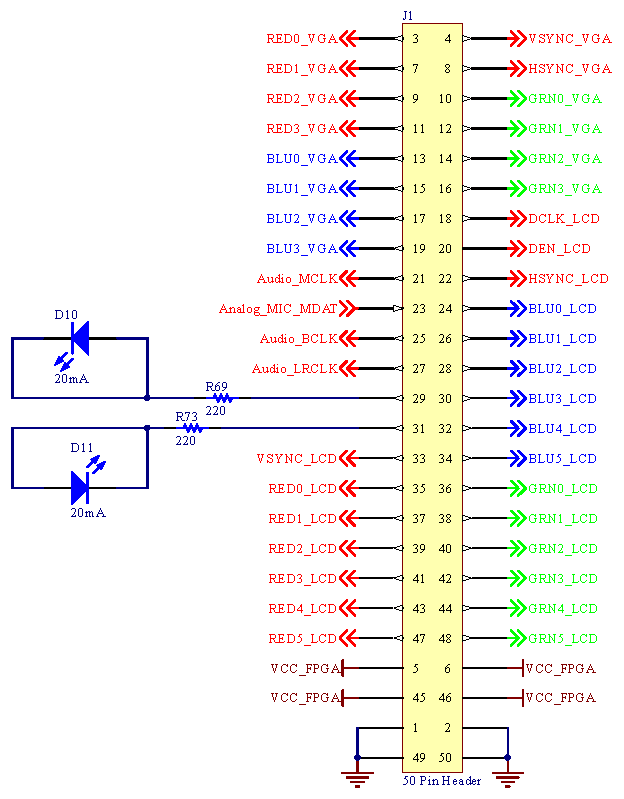
\includegraphics[width=0.5\linewidth]{Figures/50_pin_header.pdf}\centering
	\caption{Schematic of 50-pin Header}
	\label{fig:header}
\end{figure}

\subsection{Power Control Circuitry}
\label{chap:batt}
	The Power Control circuitry was designed to ensure that certain devices could be switched off if required, and also to ensure that adequate power was being supplied to all necessary components on the device. 
To begin a number of voltage regulators were added to the schematic as well as a flip-flop to be used for the main FPGA power. 
A I2C I/O Expander was also used in the schematic so that all the voltage regulators could be connected to it.\\

	The circuitry was connected up by first connecting a slide switch between the shutdown and power lines of the voltage regulator. 
An LED was then connected to the output line to ensure that if the regulator was powered an LED would illuminate, with the output line producing the required power rail needed. 
This was repeated six times to create the multiple power rails required for all the different components.\\

	There were a few changes made to the power control circuitry after going through and analysing all the schematics. 
It was found that the voltage regulator would only give out 0.1A of current whereas the modems would need at least 2A of current, 4A at best. 
The circuitry was updated to include the new part found so that the output current would be adequate for the modems. \\

\subsection{Charging Circuitry}

	The charging circuit was designed using a Bq25071 chip connected to a MicroUSB connector. 
The charging circuit chip was set to be powered by the battery voltage line. The circuitry was designed following the datasheet of the IC.
Figure \ref{fig:charger} displays the charging circuit with the MicroUSB connection to the left. 

\begin{figure}
	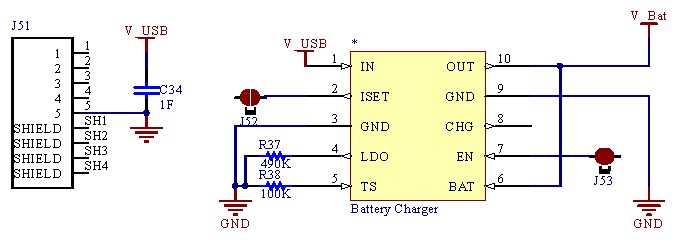
\includegraphics[width=0.5\linewidth]{Figures/battery_charger.pdf}\centering
	\caption{Schematic of Charging Circuit with MicroUSB connection}
	\label{fig:charger}
\end{figure}

\subsection{Voltage Step-Up \& Step-Down}

	The Voltage Step-up was required as a few of the components require 5V. 
This was completed by using an NCP1402 and connecting VCC MIC to the input voltage line. 
The rest of the circuitry was completed by following the recommended layout in the data sheet. 
The use of the NCP1402 was based on a recommendation written in a past student's thesis, with the component being verified for its usability in the phone. 
An LP5951 was used to step the voltage down from 3.3V to 1.3V for the required components which needed this voltage. 
Figures \ref{fig:stepup} and \ref{fig:stepdown} display the schematics for both the voltage step-up and step-down circuits.

\begin{figure}
	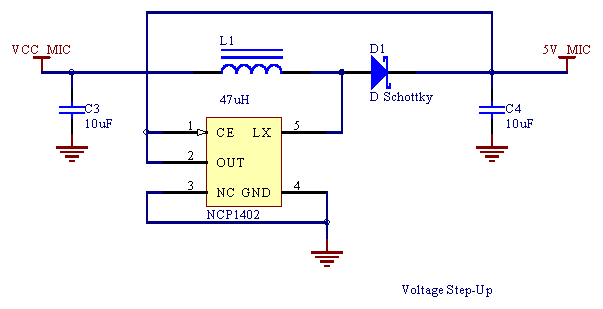
\includegraphics[width=0.5\linewidth]{Figures/voltage_stepup.pdf}\centering
	\caption{Schematic of Voltage Step-Up}
	\label{fig:stepup}
\end{figure}

\begin{figure}
	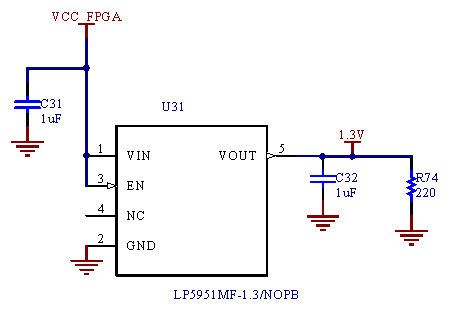
\includegraphics[width=0.5\linewidth]{Figures/voltage_stepdown.pdf}\centering
	\caption{Schematic of Voltage Step-Down}
	\label{fig:stepdown}
\end{figure}

\subsection{Signal Connections}

	The Signal Connections schematic was designed to contain all the off-sheet connectors from the various components which operated through I2C and Interrupt lines. 
The separate signals were connected together with resistor pull-ups added to the two I2C lines. 
The output of these signals were all sent directly to FPGA pins. 
Figure \ref{fig:SCL} displays the schematic for the SCL connections. 

\begin{figure}
	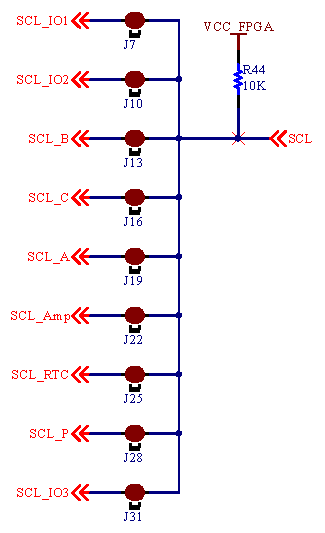
\includegraphics[width=0.5\linewidth]{Figures/SCL_lines.pdf}\centering
	\caption{Schematic of SCL connections}
	\label{fig:SCL}
\end{figure}


\subsection{I2C I/O Expanders}

	There were a number of I/O Expanders which were added to the device. These were added to add in a number of peripherals which didn't necessarily need to be connected to FPGA pins. There were a number of expanders due to all the pins on a particular expander needing to have the same inout/output source. 
The I/O Expanders were added into the schematics to allow the device to have more connections. The DPAD and buttons were connected to an I/O Expander with the use of resistor pull-ups. A number of other signals which were required to be active while the FPGA was active, were added to another I/O Expander.
Figure \ref{fig:I2C} displays the schematic for one of the I2C Expanders. 

\begin{figure}
	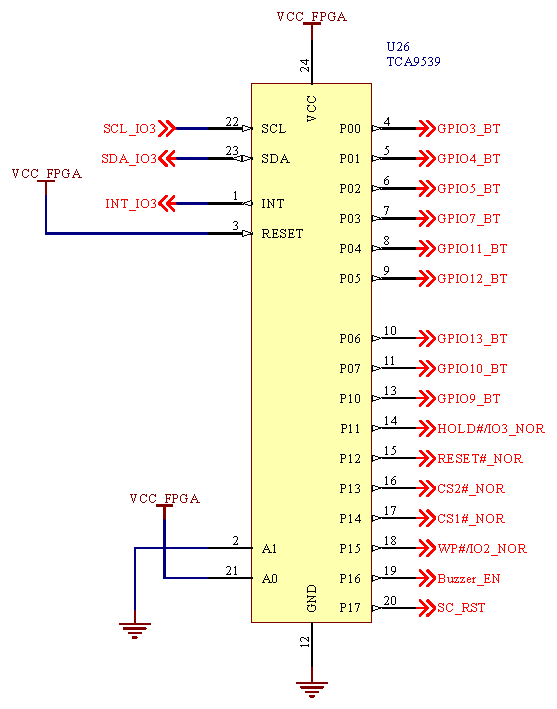
\includegraphics[width=0.5\linewidth]{Figures/I2C_Expander.pdf}\centering
	\caption{Schematic of I2C Expander}
	\label{fig:I2C}
\end{figure}

\subsection{VGA Connection}
\label{chap:VGA}

	The VGA was connected using a 15-Pin DSUB connector. 
A resistor ladder was used for the colour connections with the signals going straight out to the FPGA board.
Resistor values of 4k, 2k and 510 Ohms were used for the ladder with two 0 Ohm resistors used for the HSYNC and VSYNC lines. 
The data sheet for the VGA connection was used as a basis for the signal connections. 
Figure \ref{fig:VGA} displays the VGA connection. 

\begin{figure}
	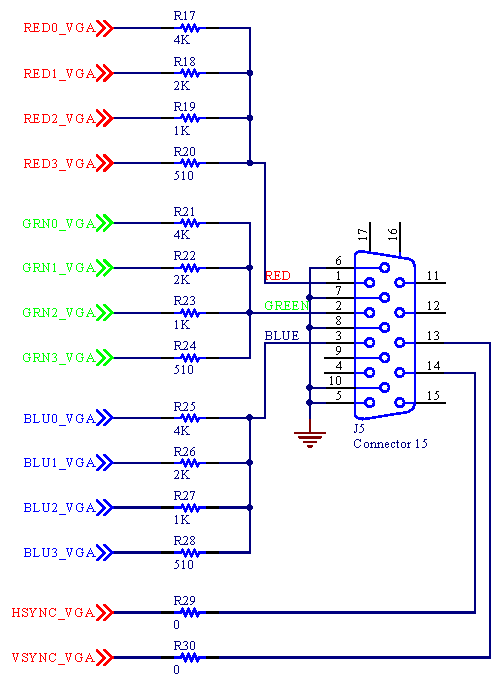
\includegraphics[width=0.5\linewidth]{Figures/VGA.pdf}\centering
	\caption{Schematic of VGA Connection}
	\label{fig:VGA}
\end{figure}

\subsection{LCD Display}
\label{chap:LCD}

	The LCD Display schematic was connected in a similar way as the VGA connection with resistor pull-ups used for all three colour connections. 
The purpose of the schematic would be to provide the LCD display for the phone.
Figure \ref{fig:LCD} displays the LCD connection.

\begin{figure}
	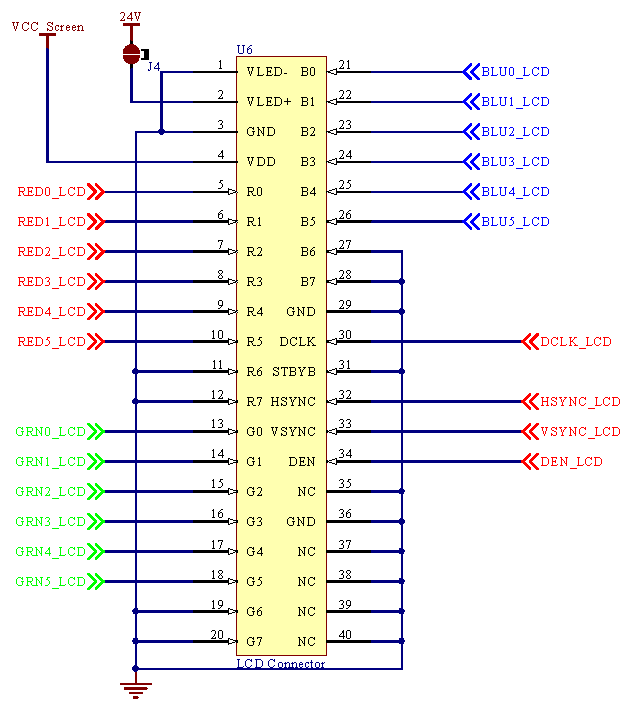
\includegraphics[width=0.5\linewidth]{Figures/LCD.pdf}\centering
	\caption{Schematic of LCD Screen Connection}
	\label{fig:LCD}
\end{figure}

\subsection{Touch Screen}
\label{chap:touch}

	The Touch Screen was added to the schematic to give the ability to the user to use their fingers for functionality, as well as the thumb-pad and buttons. 
The Touch Screen connection was completed by powering it with VCC Screen and adding in I2C signals and an Interrupt line, going to the Signal Connections sheet.

\subsection{LED Backlight Display}

	The LED Backlight Display was designed using a simplified design already created by another producer. This circuit was designed to provide a back lit display when the phone is on and to dim the screen when the phone is in a call or facing down.
Figure \ref{fig:backlight} displays the LED Backlight connection. 

\begin{figure}
	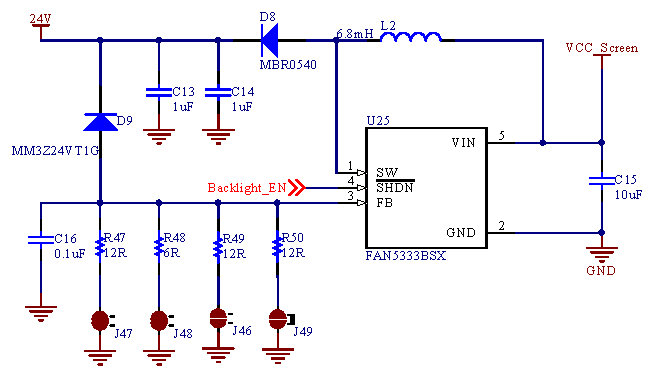
\includegraphics[width=0.5\linewidth]{Figures/LED_backlight.pdf}\centering
	\caption{Schematic of the LED Backlight Connection}
	\label{fig:backlight}
\end{figure}

\subsection{Accelerometer}
\label{chap:a}

	The accelerometer was designed mainly through reading the recommended application layout in the data sheet of the component. Off-sheet connectors were used for the I2C signals and the Interrupt lines, as well as the three ADC lines which were used for the volume thumb wheel. The power for the component was connected to the VCC MIC power rail.
Figure \ref{fig:a} displays the accelerometer connection. 

\begin{figure}
	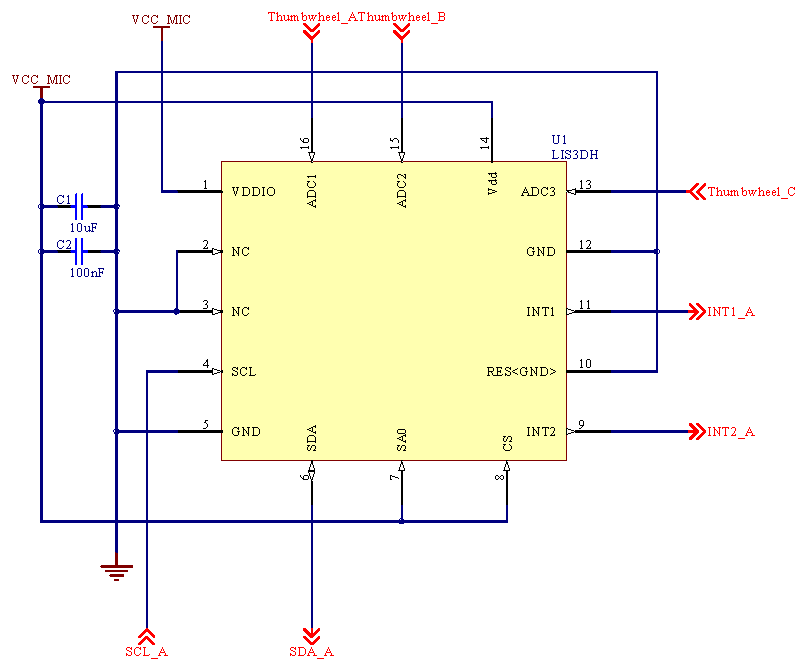
\includegraphics[width=0.5\linewidth]{Figures/accelerometer.pdf}\centering
	\caption{Schematic of the Accelerometer Connection}
	\label{fig:a}
\end{figure}

\subsection{Real-Time Clock}
\label{chap:RTC}

	The schematic connections for the RTC were made by following the typical application layout given in the manufacturer's data sheet.
Figure \ref{fig:RTC} displays the real-time clock connection. 

\begin{figure}
	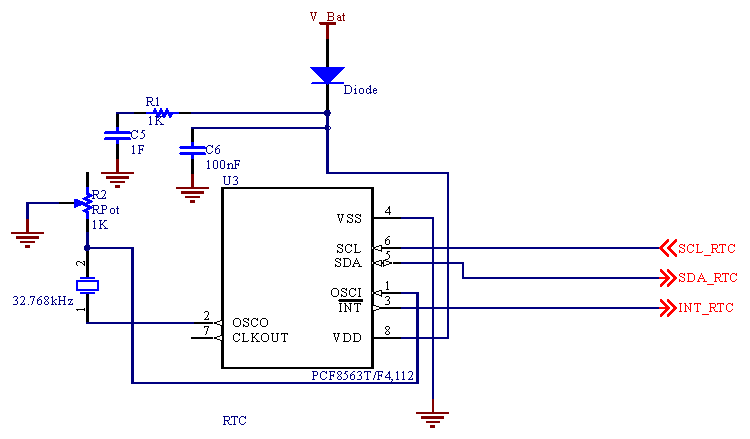
\includegraphics[width=0.5\linewidth]{Figures/RTC.pdf}\centering
	\caption{Schematic of the Real-Time Clock Connection}
	\label{fig:RTC}
\end{figure}

\subsection{Proximity Sensor}
\label{chap:prox}
	The schematic and PCB models for the Proximity Sensor were accessed from the internet with all the connections followed from the manufacturer's data sheet. 
Figure \ref{fig:prox} displays the proximity sensor connection. 

\begin{figure}
	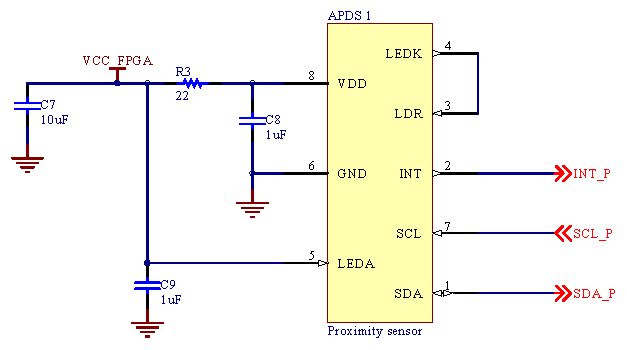
\includegraphics[width=0.5\linewidth]{Figures/prox_sensor.pdf}\centering
	\caption{Schematic of the Proximity Sensor Connection}
	\label{fig:prox}
\end{figure}

\subsection{4G Modems}
\label{chap:modem}

	4G modems were added to the device to enable 4G internet connection. 
Two 4G modems were added to the schematics so that the user would have the ability to be connected to two different networks at once.
The schematic for the 4G modem was downloaded off the internet with many of the connections also being read off the manufacturer's data sheet. 
Figure \ref{fig:modem} displays the 4G modem connection. 

\begin{figure}
	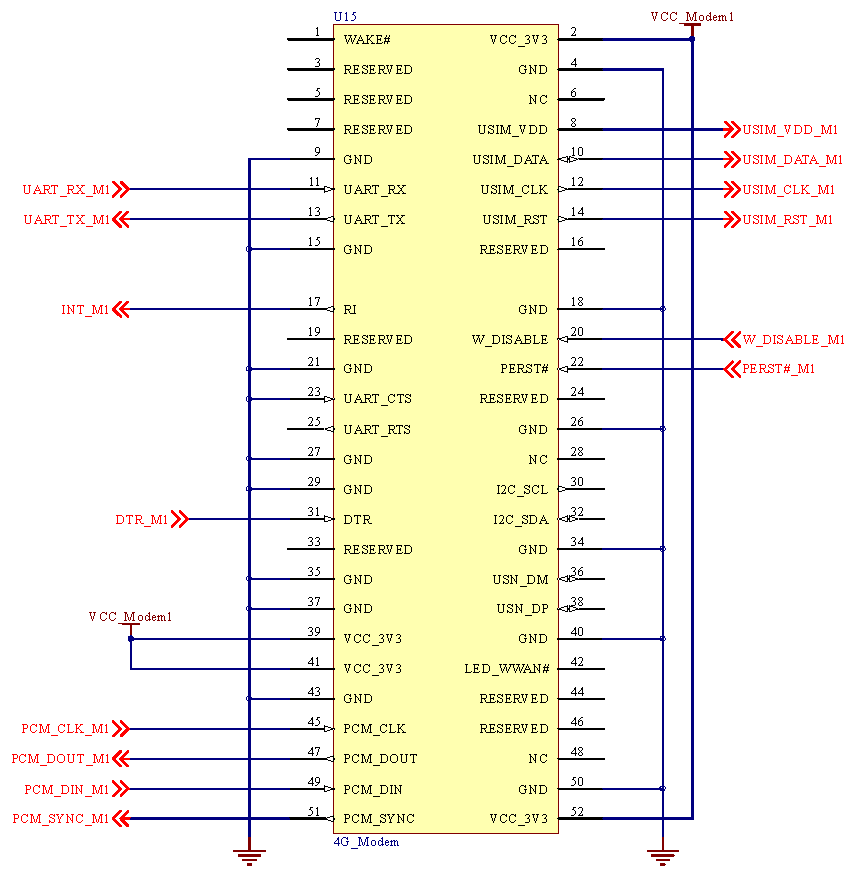
\includegraphics[width=0.5\linewidth]{Figures/modem.pdf}\centering
	\caption{Schematic of the 4G Modem Connection}
	\label{fig:modem}
\end{figure}

\subsection{WiFi Module}

	The WiFi module was added into the schematics to enable the phone to have WiFi capability. This module was connected through the GPIO bits and an I2C connection.

\subsection{NOR Flash}

	The NOR Flash schematic was designed to have primary use within the One-Time Pad encryption. The component would have no other function on the phone. 

\subsection{Barometer}

	The schematic connections for the Barometer were completed by following the recommended layout given on the manufacturer's data sheet. 
Figure \ref{fig:barometer} displays the schematic for the barometer. 

\begin{figure}
	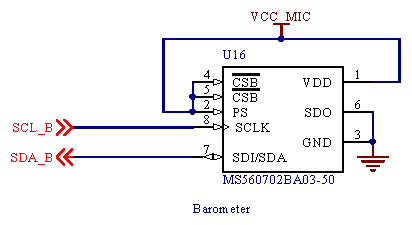
\includegraphics[width=0.5\linewidth]{Figures/barometer.pdf}\centering
	\caption{Schematic of the Barometer}
	\label{fig:barometer}
\end{figure}

\subsection{LoRa Radio}

	The two LoRa Radios were connected up using the recommended application layout given by the manufacturer's data sheet. 
The UART connections were made directly to the FPGA pins. 

\subsection{MEMs Microphones}
\label{chap:mics}

	The two MEMs Microphones were connected by following the data sheet's guidelines. The individual data lines were sent straight to the FPGA, while the two clock lines were tied together and sent to the FPGA board. 

\subsection{Headphone Audio Filter} 
\label{chap:audio2}

	The Headphone Audio Filter was created by following the design of a Sallen-Key Lowpass Filter, with two being designed. A chip containing two amplifiers was used for the design with the output of both chips being the left and right headphone audio respectively. 

\subsection{Audio Power Amplifier}
\label{chap:audio}

	The schematic for the Audio Power Amplifier was completed using a number of recommended layouts found in the component's recommend layout and recommended schematics found across the internet. This schematic was designed to produce the audio for the phone. 
Figure \ref{fig:audio} displays part of the audio circuitry. 

\begin{figure}
	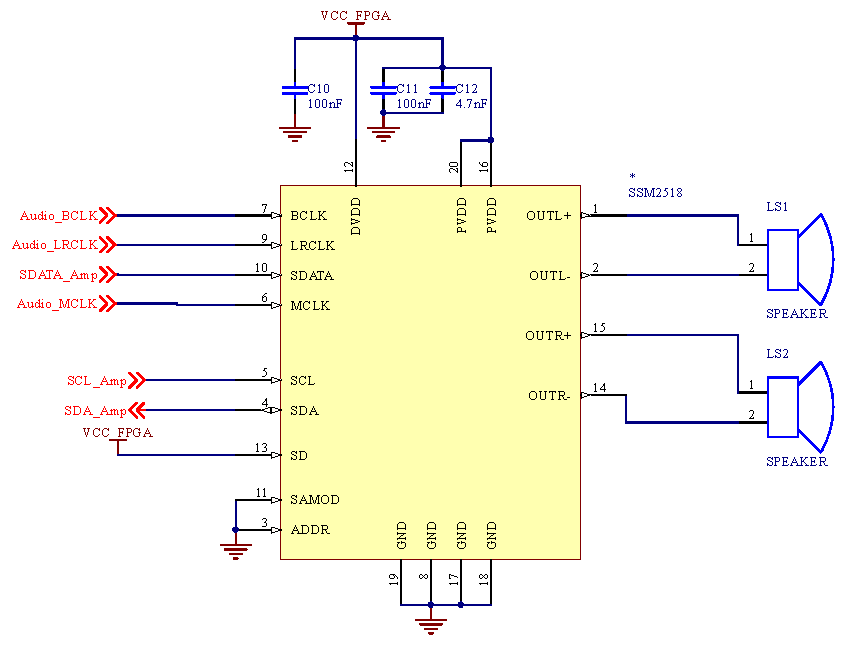
\includegraphics[width=0.5\linewidth]{Figures/audio_circuitry.pdf}\centering
	\caption{Schematic of part of the Audio Circuitry}
	\label{fig:audio}
\end{figure}

\subsection{Digital Compass}

	The Digital Compass was added to give the device the use of a compass which would be used for both gyroscopic effect and the location of the device.
Like many of the other components the signal connections on the schematic were wired using the recommended application layout. 
Figure \ref{fig:compass} displays the schematic of the digital compass. 

\begin{figure}
	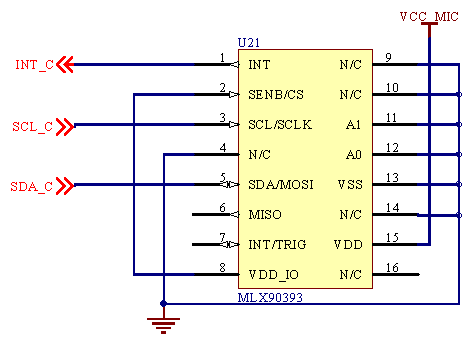
\includegraphics[width=0.5\linewidth]{Figures/compass.pdf}\centering
	\caption{Schematic of the Digital Compass}
	\label{fig:compass}
\end{figure}

\subsection{Bluetooth Module}

	The Bluetooth module was added into the schematic to ensure that the device would be compatible with Bluetooth. This would allow the user to connect to a third-party peripheral device.
The circuitry for the Bluetooth module was created by following the recommend layout on the component's data sheet. The UART and PCM connections were made directly to FPGA pins. 

\subsection{SIM Card Connection}
\label{chap:SIM}

\subsection{MicroSD Card Slot}
\label{chap:SD}

	The MicroSD connection was created by downloading a MOLEX schematic and footprint from SnapEDA. The data, clock and chip select lines were connected to the FPGA directly with a 100k$\Omega$ pull-up resistor for every signal. The structure for the pull-up resistors was followed from a Nexys 4 DDR schematic sheet created by Digilent. 

\subsection{Smart Card Connection}
\label{chap:SC}

	The Smart Card Connection was created by designing a custom footprint and schematic. 
The footprint was drawn based off the Smart Card Slot datasheet, with the schematic being a basic header block with ten connections.\\
The Smart Card was implemented to allow the user to make payments with their phone, without having to pull out their credit/debit card.
Figure \ref{fig:SC} displays the schematic for the Smart Card Connection. 

\begin{figure}
	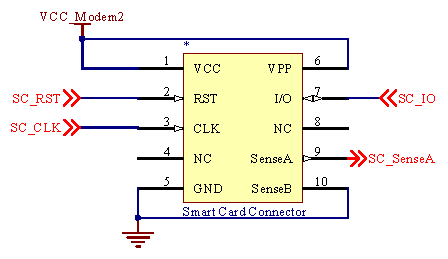
\includegraphics[width=0.5\linewidth]{Figures/SC.pdf}\centering
	\caption{Schematic of the Smart Card Connection}
	\label{fig:SC}
\end{figure}

\subsection{Buzzer}
\label{chap:buzzer}

	The buzzer was added to allow notifications whenever a text or missed call was recieved.
Figure \ref{fig:buzzer} displays the schematic for the buzzer. 

\begin{figure}
	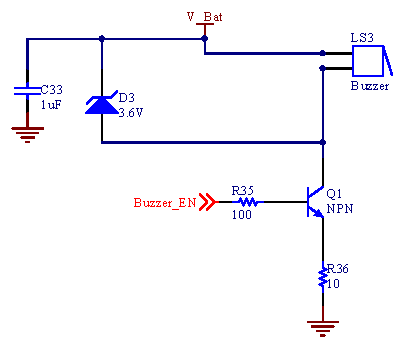
\includegraphics[width=0.5\linewidth]{Figures/buzzer.pdf}\centering
	\caption{Schematic of the Buzzer Connection}
	\label{fig:buzzer}
\end{figure}

%----------------------------------------------------------------------------------------


 
% Chapter 6

\chapter{Schematic \& PCB Layout} % Main chapter title

\label{Chapter6} % For referencing the chapter elsewhere, use \ref{Chapter1} 

\AddToShipoutPicture*{\SchematicLayout}

\begin{parcolumns}[colwidths={1=.6\textwidth},rulebetween=false]{2}
\colchunk{% left column

%----------------------------------------------------------------------------------------
	This section provides a detailed overview of the process and findings of the circuit designs to create the schematic designs, as well as the derivation of the PCB from the schematic designs.
This includes: (\ref{chap6sec1} the schematic design errors and (\ref{chap6sec2}) testing, (\ref{chap6sec3}) PCB concept drawings, (\ref{chap6sec4}) the PCB footprint design, (\ref{chap6sec5}) the layout of the PCB, (\ref{chap6sec6}) the routing of the PCB and (\ref{chap6sec7}) any major challenges which were faced.\\
For the full schematic designs see Appendix \ref{AppendixA} and for the full PCB layout see Appendix \ref{AppendixB}.\\

}
\colchunk{% right column
}
\end{parcolumns}
\newpage

%----------------------------------------------------------------------------------------
%	SECTION 1
%----------------------------------------------------------------------------------------

\section{Errors in the Schematic Designs}
\label{chap6sec1}

There were originally as many as 900 errors found in the design project after compiling. 
A large number were removed by disabling the warning given for off-grid objects. 
This left about 500 errors which needed to be solved individually. 
The following list describes the major errors and how they were solved.

\begin{itemize}
\item no driving source; this was corrected in a number of different ways. 
In some situations it required signal connections at each end to be related (input to output) and not the same. 
In other cases it required adding in either a power rail or a ground to the affected component to fix the driving source. 
\item only one pin connection; this was solved by going to the causing net label, recreating it and placing it in the desired location. 
\item a certain component had a mix of I/O pins and output pins (or power pins); this was solved by changing the pin types of the affecting pins to match the required in type. 
This was an easy solve in most cases however some were more tricky and required work overall several schematics. 
\end{itemize}

A few other small changes were made to the schematics to improve the aesthetic and readability of the documents, as well as saving the amount of components needed. 
All of the resistor pull-ups for the I2C connections were moved to the Signal Connections schematic, which saved a large number of resistors and space. 
Also, the solder jumpers were removed and replaced with ones which were professionally created, so that they would give no errors.

%----------------------------------------------------------------------------------------
%	SECTION 2
%----------------------------------------------------------------------------------------

\section{Testing the Schematic Components}
\label{chap6sec2}

The initial testing was started before the schematic were completed and before the design of the PCB. 
The first components which were tested were the voltage regulators and the flip-flops being used within the Power Control circuitry. 
It was vital that the correct voltage was being read out of the flip-flop to ensure that the correct pins were being wired. 
It was also vital that the correct lines were being shutdown if necessary so that the security of the circuitry could be verified. 
The circuitry was put together and tested on a small breadboard with both a resistor and a capacitor in certain positions to obtain the required voltage. 
Once the expected reading was achieved the circuit was copied into the schematic for the Power Control circuitry and was replicated a number of times for all the required power rails. 
Figure \ref{fig:power_circuit} shows the power circuit used with the smaller IC being the voltage regulator and the larger IC being the flip-flop.

\begin{figure}
	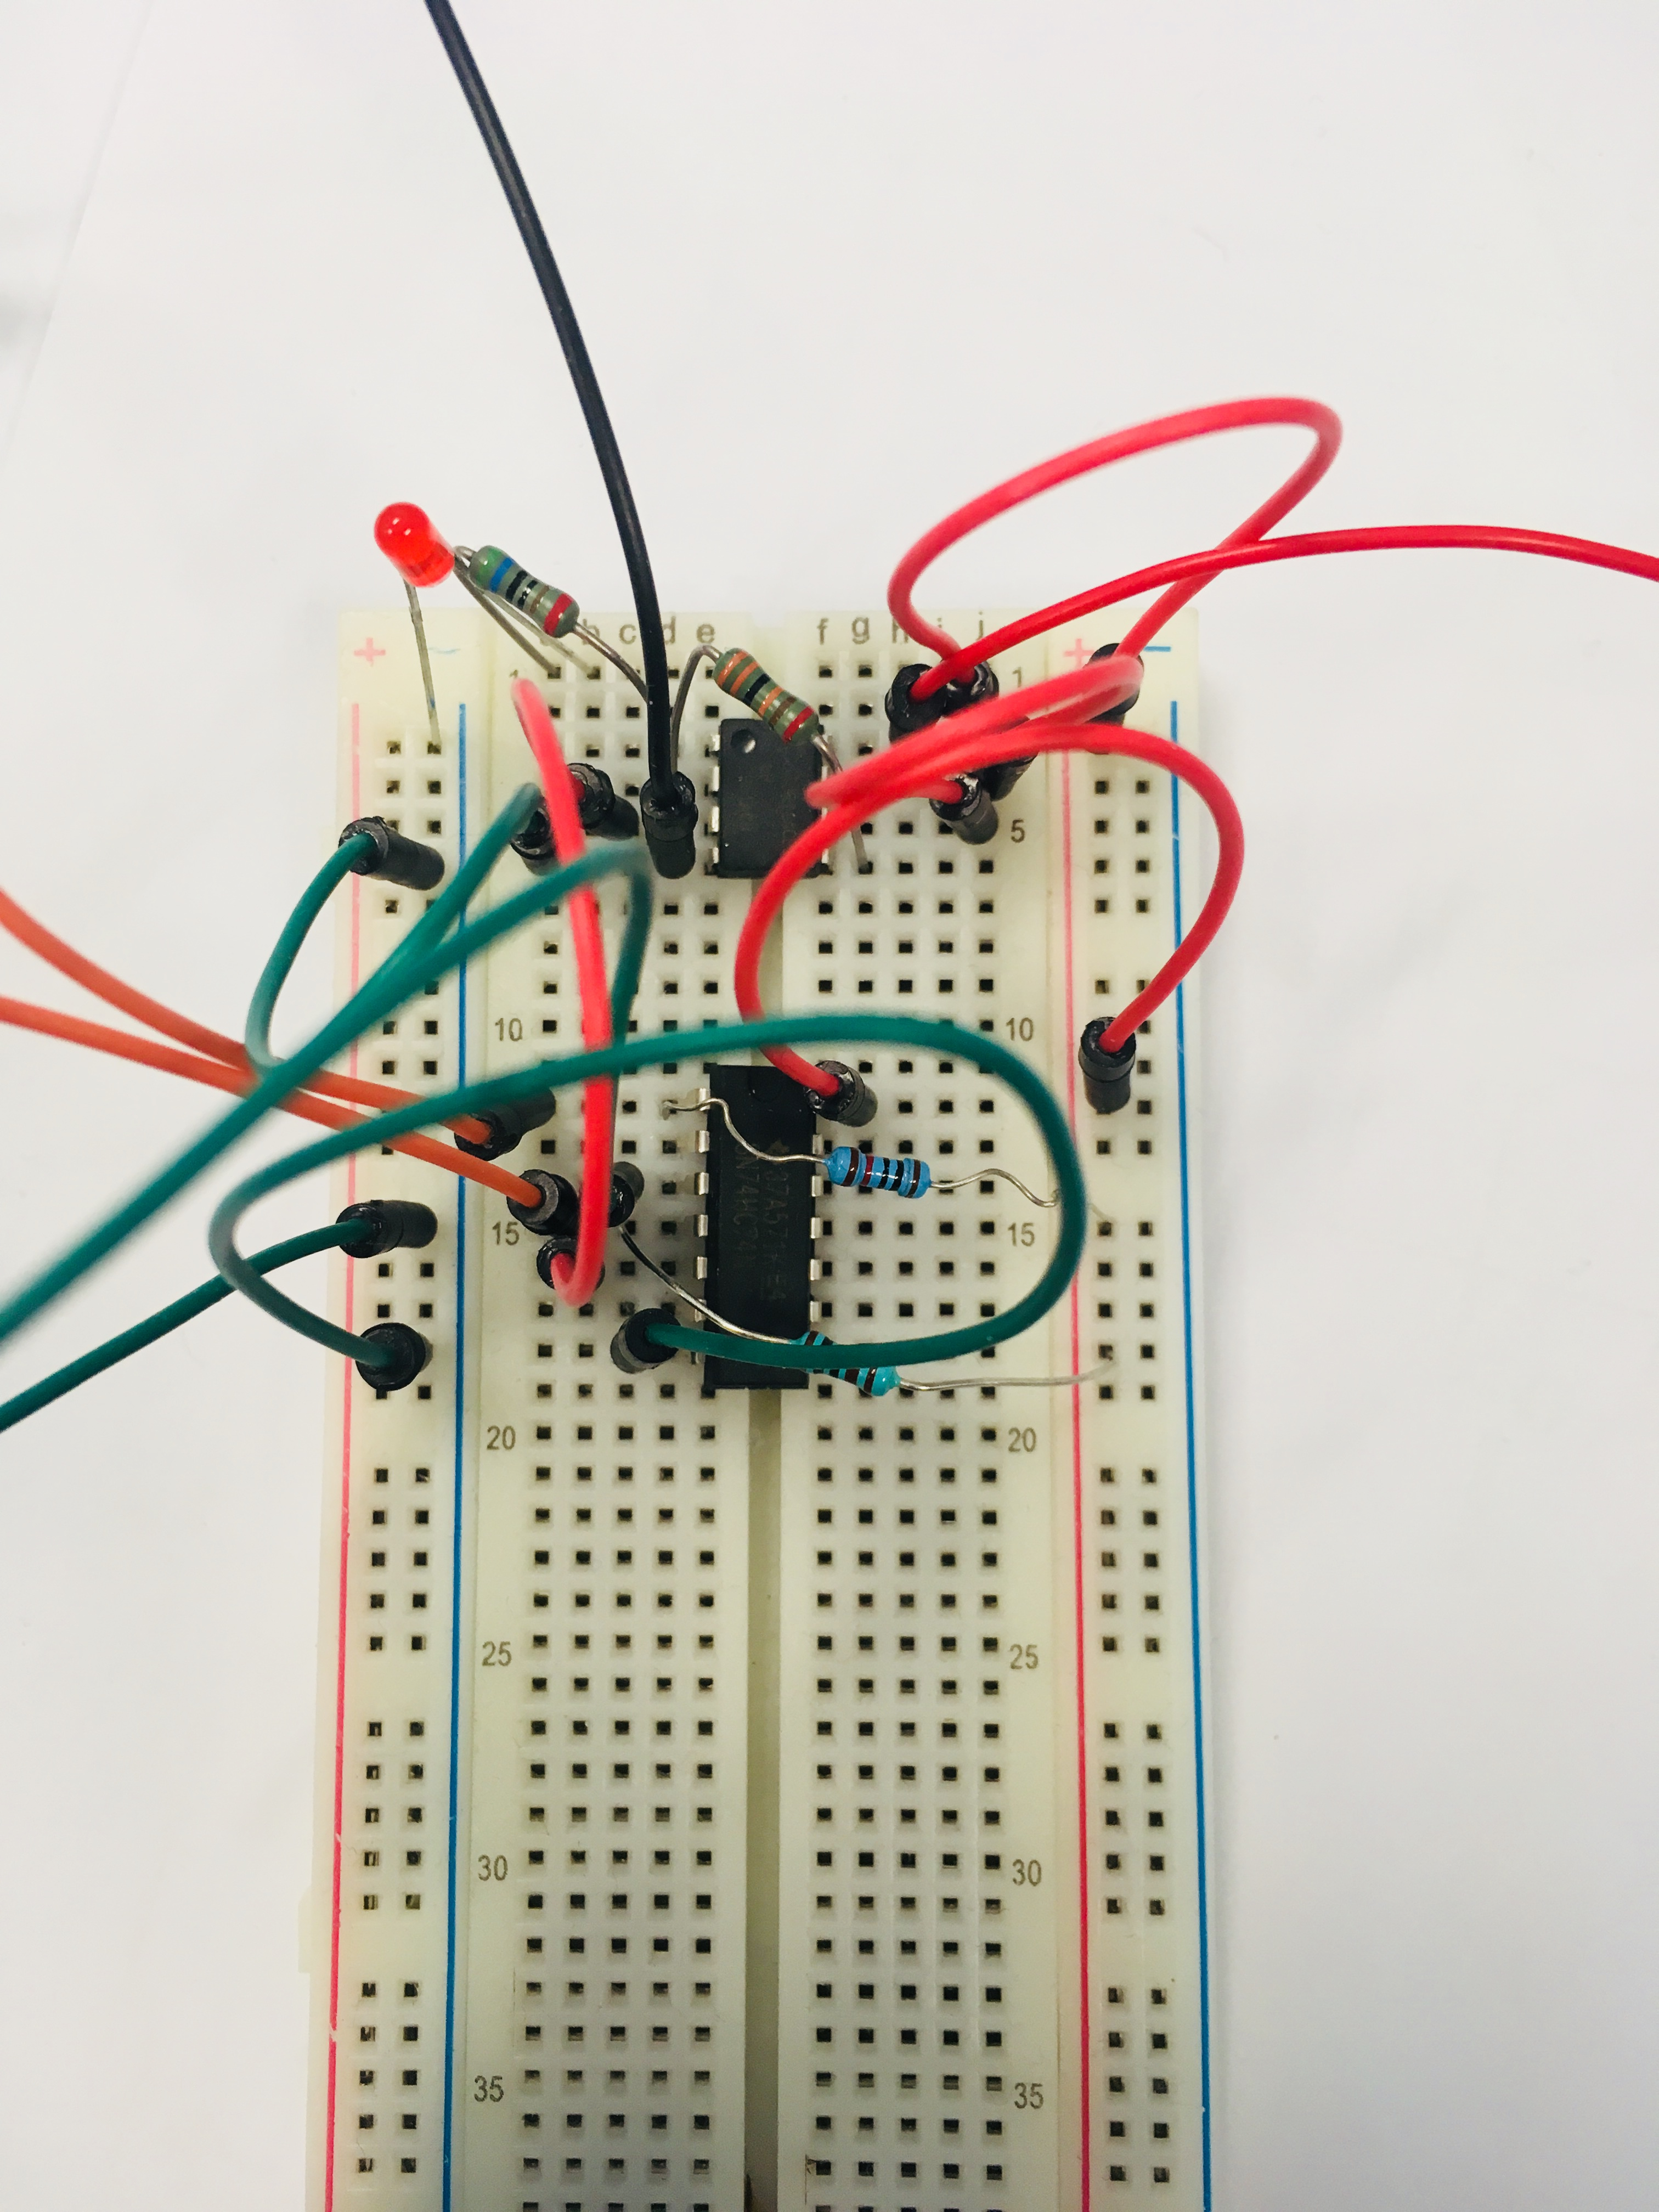
\includegraphics[width=0.5\linewidth]{Figures/powercircuit.jpg}\centering
	\caption{Image of test power circuit}
	\label{fig:power_circuit}
\end{figure}


%----------------------------------------------------------------------------------------
%	SECTION 3
%----------------------------------------------------------------------------------------

\section{PCB Concept}
\label{chap6sec3}

The PCB layout originated from early concept designs created by Paul Gardner-Stephen. 
This multi-layered design was used to visualise the placement of every major component within the phone.
Figure \ref{fig:Concept} displays the concept design on the top layer. 

\begin{figure}
	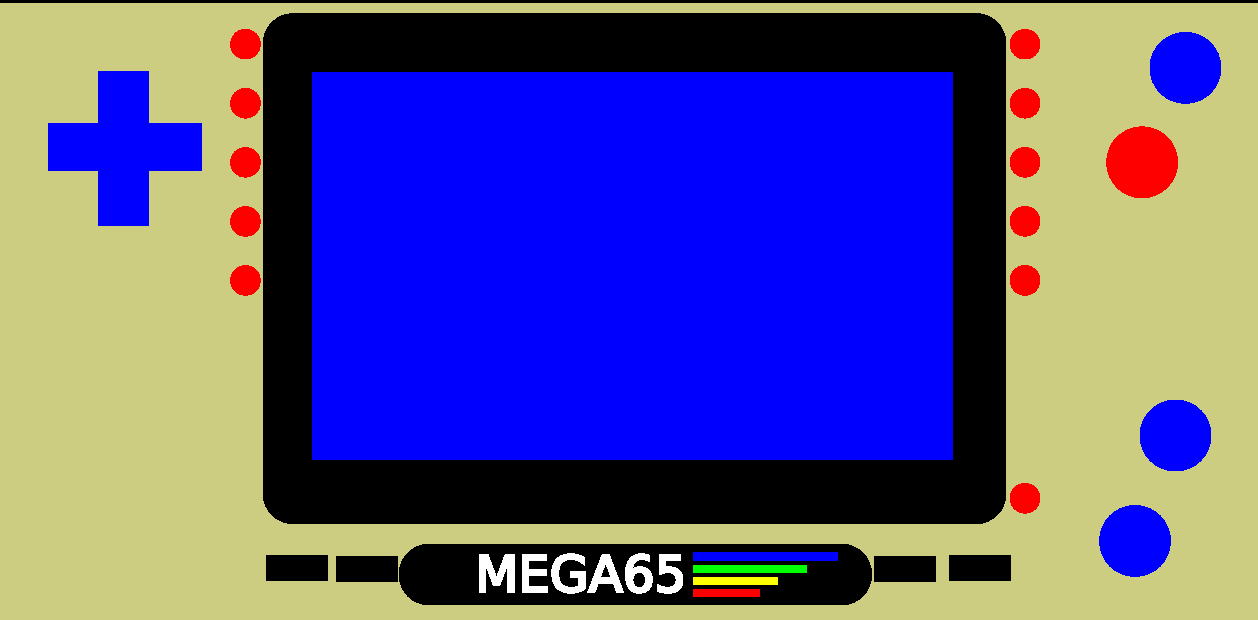
\includegraphics[width=\linewidth]{Figures/handset-layout-v1.pdf}
	\caption{Initial PCB Concept}
	\label{fig:Concept}
\end{figure}

	The following figures display the lower layers of the concept, detailing the location of most of the vital components. 

\begin{figure}
	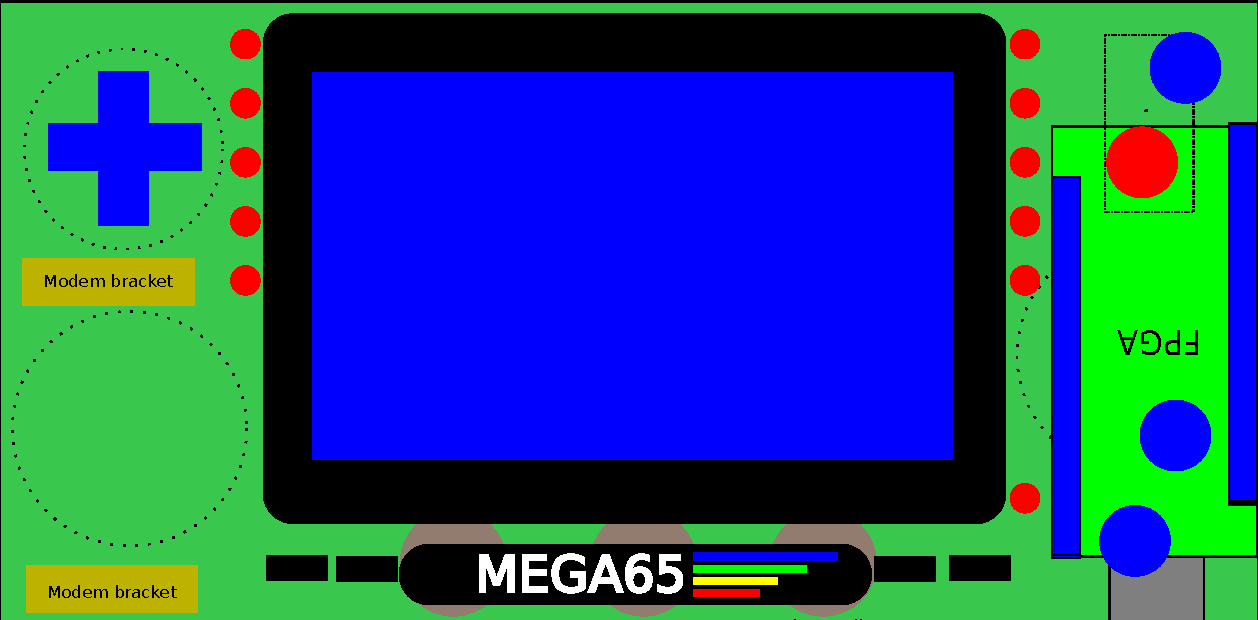
\includegraphics[width=\linewidth]{Figures/handset-layout-v1-no-Cover.pdf}
	\caption{Concept PCB with no cover}
	\label{fig:nocover}
\end{figure}

\begin{figure}
	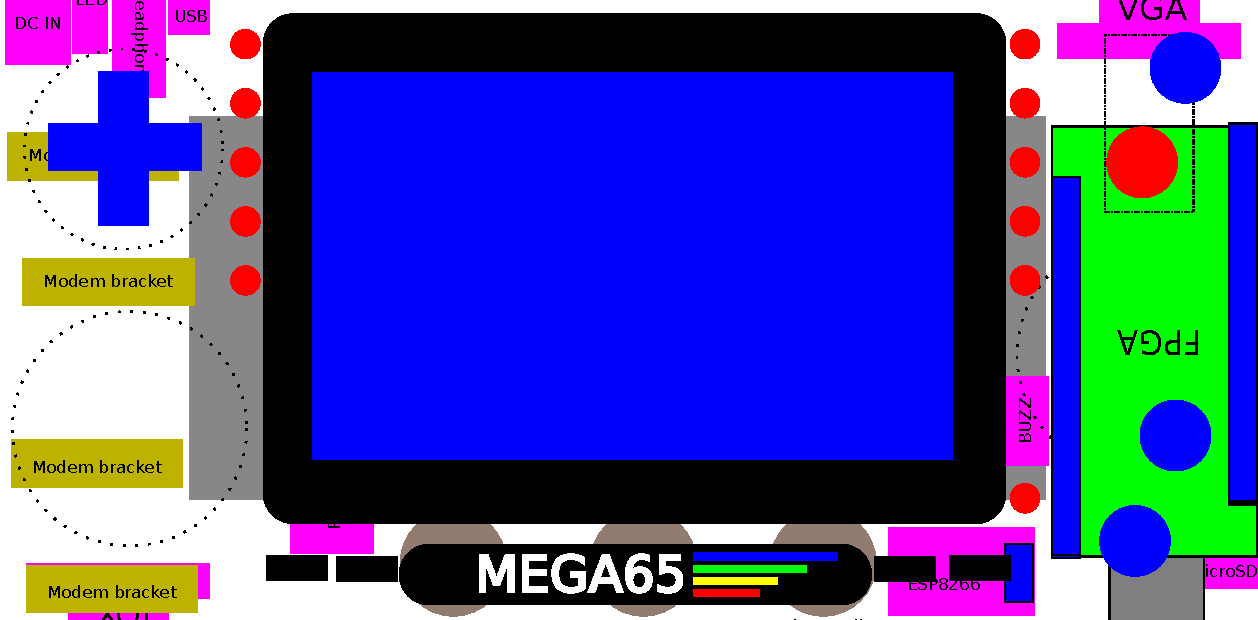
\includegraphics[width=\linewidth]{Figures/handset-layout-v1-no-PCB-no-Cover.pdf}
	\caption{Concept detailing PCB component placement }
	\label{fig:nopcb}
\end{figure}

%----------------------------------------------------------------------------------------
%	SECTION 4
%----------------------------------------------------------------------------------------

\section{PCB Footprint Design}
\label{chap6sec4}

	Most of the components were either downloaded from the manufacturer's approved source (eg. Digikey) or SnapEDA, components which didn't have footprints or where the footprints had incorrect dimensions were created manually using the footprint editor in Alitum. 
The footprints were created by following the recommended PCB outline in the desired component's datasheet. 
There were a few components where the datasheet was unavailable and hence the footprints were created using precise measurements of the actual item. 
The following list describes the footprints which were created without a datasheet, and how they were created;

\begin{itemize}
\item The footprints for the silicon moulds for the push buttons were designed in Altium using a pre-existing official footprint used for the design of the Nintendo GameBoy. 
This larger footprint was modified into the separate components of the DPAD buttons, the blue push buttons and the rectangular black push buttons.
\item The footprint for the modem connector was created by measuring the dimensions of the physical component. 
This connection part was then added to the recommended PCB layout of the modem, which was created from the datasheet. 
\end{itemize}

%----------------------------------------------------------------------------------------
%	SECTION 5
%----------------------------------------------------------------------------------------

\section{PCB Layout}
\label{chap6sec5}

	The start of the PCB Design process begun with a graphical editor being used to create a mock-up of the MEGA65 phone. 
This mock-up included precise measurements of the height and width of the device as well as the location of all of the major components required for the device, including the FPGA pins and the 4G Modems. 
The mock-up was used as the template for the PCB board with all of the measurements copied into the program. \\
	Once the schematic designs had been completed the PCB board was adjusted in Alitum to accommodate four layers. 
This was completed by going into Layer Stack Manager in Alitum and adding in two more signal layers. 
All of the schematic designs were then added into the PCB file and on top of the mock-up. \\
The next stage of the process involved using the mock-up (Figure \ref{fig:nopcb}) to place the required components in their suitable positions. 
This process took a while to complete as some components were required to be realigned or moved to a completely different position. 
Some component footprints also had small positioning holes, which interfered with components in the same position on the opposite side of the board. 
This also required realignment of a number of components. 
Figure \ref{fig:Initial_PCB} displays one of the initial PCB layouts of the board, before the routing stage. 
Note that this early design doesn't include a lot of the components, nor most of them are not in their correct positions.\\

\begin{figure}
	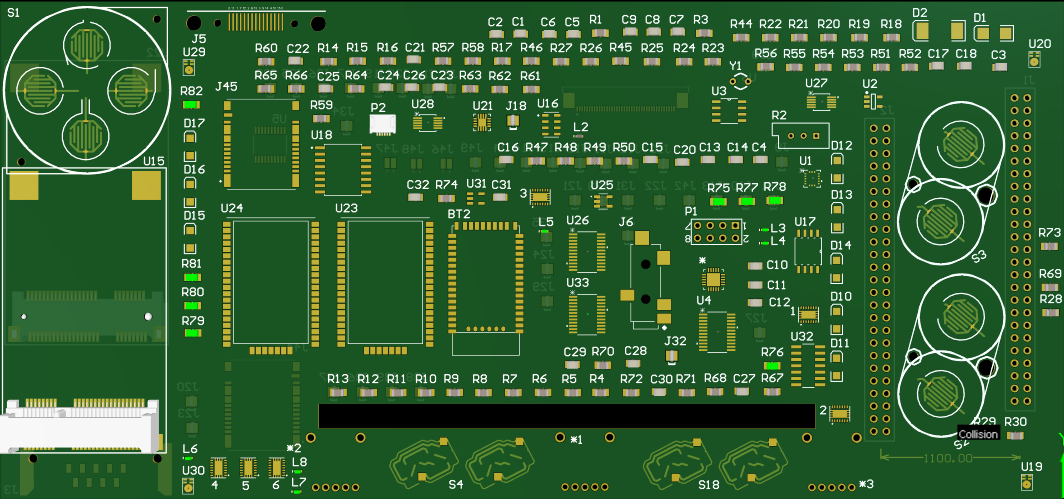
\includegraphics[width=\linewidth]{Figures/PCB.png}
	\caption{Initial PCB Layout}
	\label{fig:Initial_PCB}
\end{figure}

	It was decided near the beginning of the process that most of the ICs which would be located within the inner part of the board, would have to be positioned on the bottom layer of the board. 
This was needed to allow the LCD screen to lie flush with the board. 
It was also decided that the solder jumpers could be placed on the top side of the board below the LCD screen, as they would take up minimal height.\\

\subsection{Component Placement}
	Once all the components were placed in their relative positions they were precisely aligned into their correct positions based upon the prototype on the bench, and the concept which was made digitally. 
The FPGA pins were aligned first along with the connectors for both the LCD screen and the touch screen. 
It was essential that the large rectangular whole at the bottom of the phone was also the right width and height from the bottom of the device so that the LCD and touch ribbons would meet the connector points on the board. 
Figure \ref{fig:component_placement} shows the dimensions for the FPGA connector pins. 

\begin{figure}
	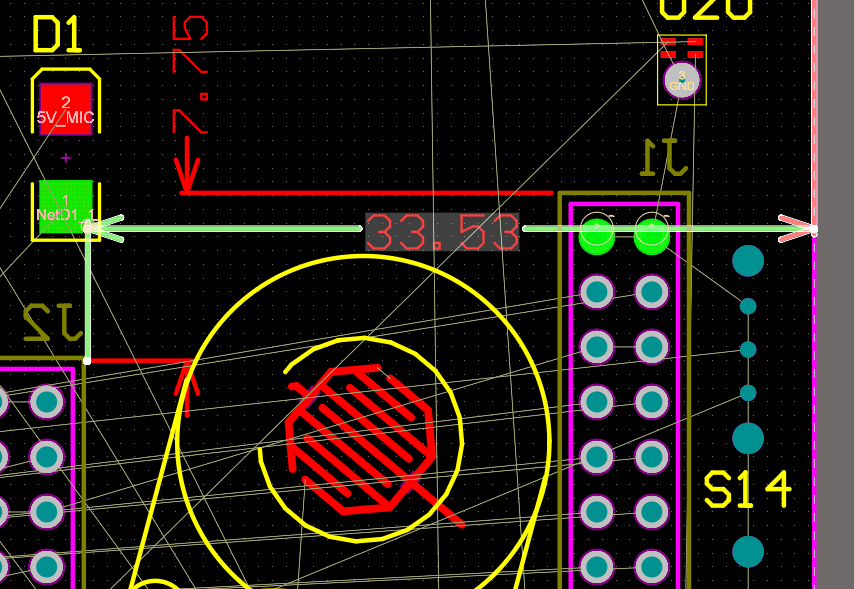
\includegraphics[width=\linewidth]{Figures/component_placement.png}\centering
	\caption{LCD Screen Dimensioning}
	\label{fig:component_placement}
\end{figure}


%----------------------------------------------------------------------------------------
%	SECTION 6
%----------------------------------------------------------------------------------------

\section{PCB Routing}
\label{chap6sec6}

	Before the routing stage of the board development could begin there were a number of errors which needed to be addressed. 
To begin, some of the footprints weren't working correctly when imported over to the PCB file. 
Some of these issues were solved by going back into the schematic files and making sure that all the correct footprints were in place, for every component. 
Another error was that there were multiple component footprints which broke the minimum track width rules. 
This was fixed by changing the track width rule settings and not include component footprints.
	To begin the routing stage of the process the rules for the PCB were defined in Altium. 
Initially the track widths and clearances were set to 0.152mm, as the lowest cheap option that can be implemented by PCBWay, and the number of layers was set to four. 
Due to the vast majority of components and sizes of some of the pads, many errors were produced concerning the minimum track widths and clearances. 
Also when routed, there were also around 160 components which were left un-routed due to the lack of space with four layers. 
This process was again tried with six layers but again the program failed to rout every component correctly. 
Finally, the track widths and clearances were set to the lowest possible dimensions able to be produced by PCBWay, this was 0.1mm. 
The number of layers on the board was also changed to eight. 
This was found to be a very expensive route for developing the board, however there were little alternatives based on the level of PCB experience. 
After completing the routing stage it was found that less than 10 connections were unable to be routed.\\
A ground plane was established within the top part of the board above the large hole, once the routing was complete. \\
Figures \ref{fig:PCB_top} and \ref{fig:PCB_bottom} display the front and back of the PCB with text boxes describing the reason for the placement of the major components. 

\begin{figure}
	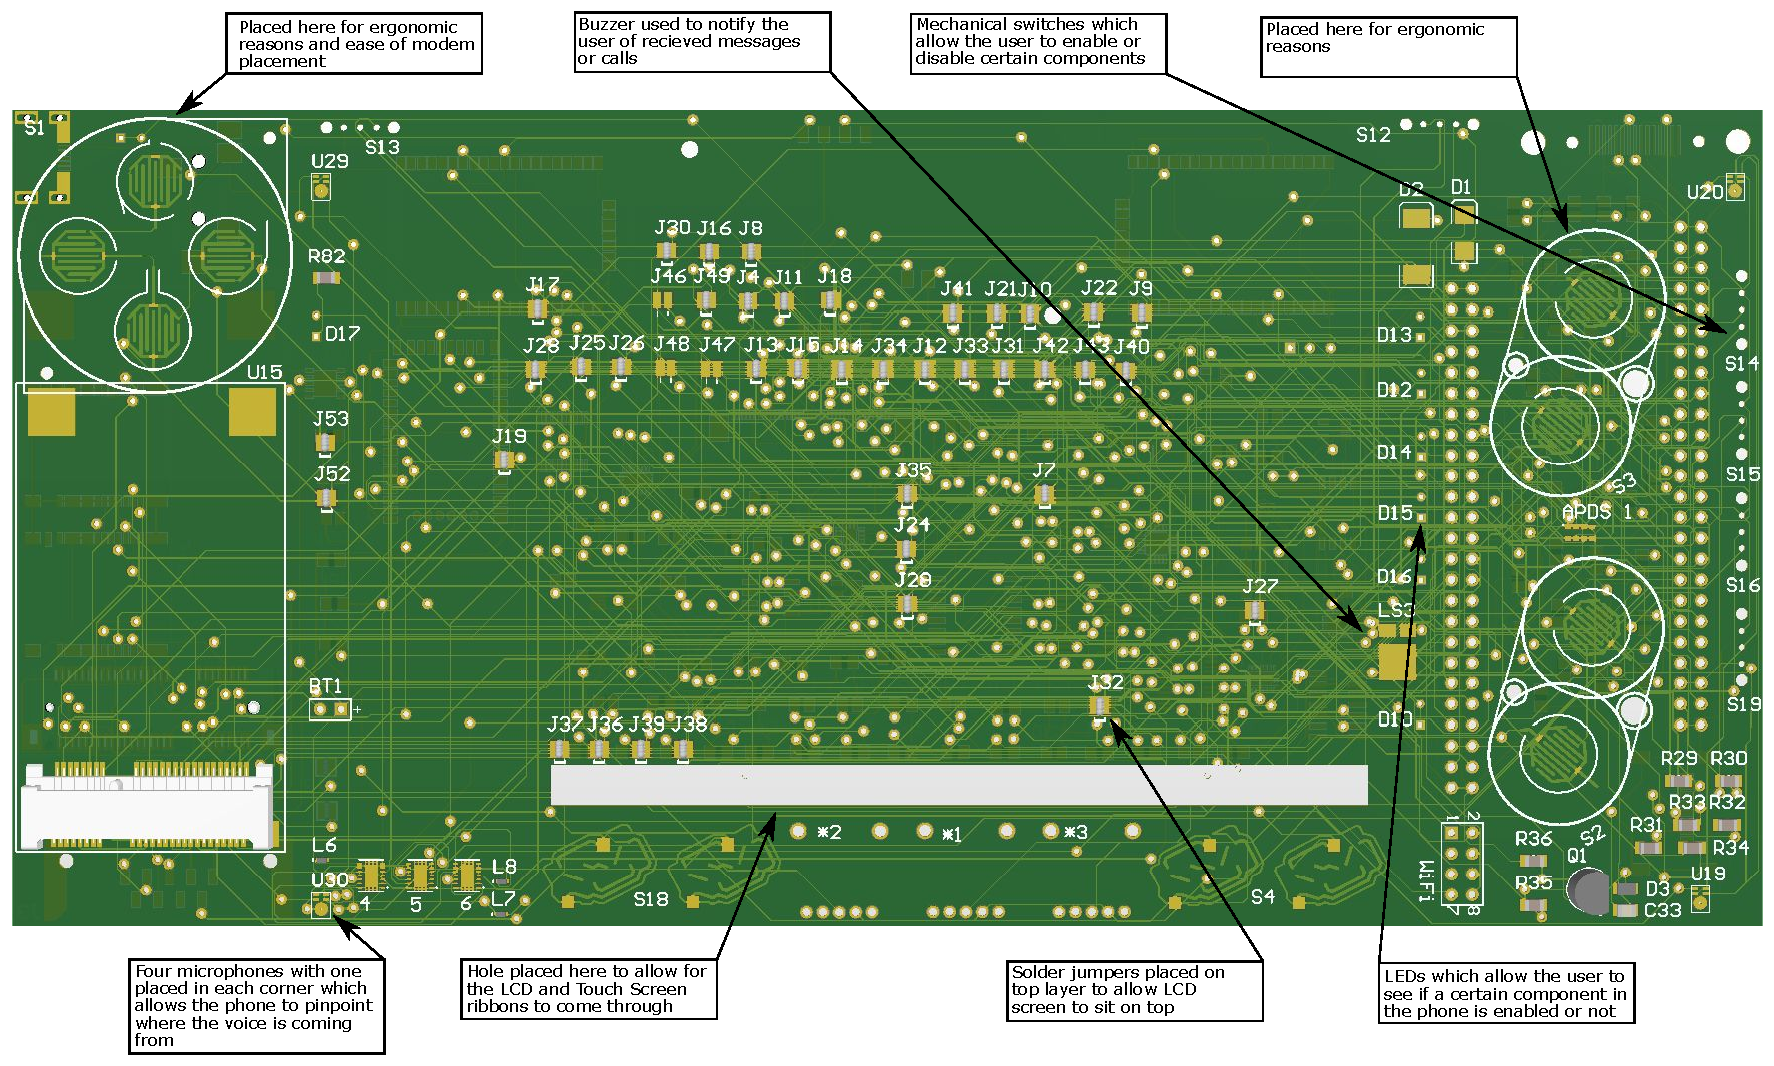
\includegraphics[angle=90, width=\linewidth]{Figures/PCB_top.pdf}\centering
	\caption{Top Side of the PCB}
	\label{fig:PCB_top}
\end{figure}

\begin{figure}
	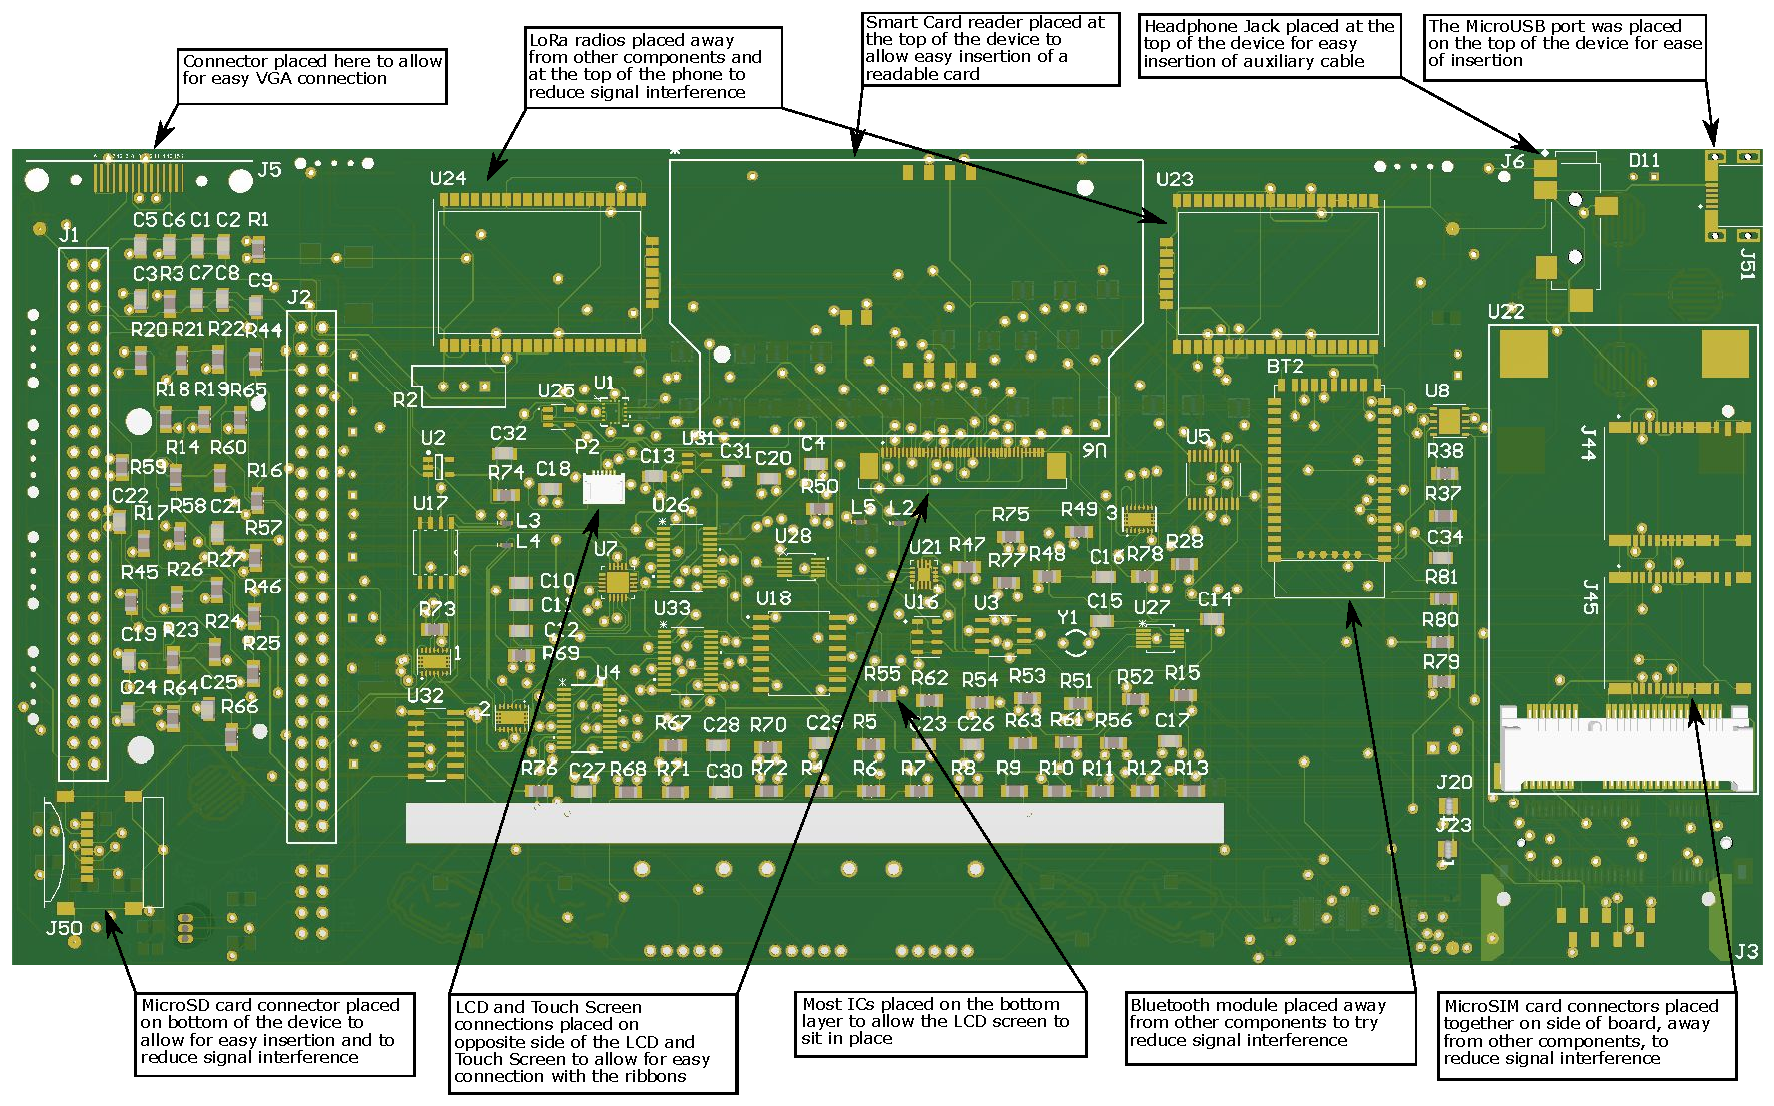
\includegraphics[angle=90, width=\linewidth]{Figures/PCB_bottom.pdf}\centering
	\caption{Bottom Side of the PCB}
	\label{fig:PCB_bottom}
\end{figure}

%----------------------------------------------------------------------------------------
%	SECTION 7
%----------------------------------------------------------------------------------------

\section{Challenges}
\label{chap6sec7}

	There were a number of challenges with designing the PCB board, mainly to do with the vast majority of components needed to be routed. 
Another challenge was discovered in the fact that the aim was to have a six-layered board, which in itself is highly sophisticated, with the finished routed board having to be eight-layered.
It was decided early on that the majority of the tricky PCB routing and design would be completed by a professional PCB designer in Germany.\\
Another challenge was found in working out the dimensions of the PCB as well as the component placement. 
Due to the size requirements of the board there was not a lot of room to spare with many components sitting flush with one another and required precise measurements to fit. \\
The PCB footprint design also provided a number of challenges with some of the components either not having datasheets, or their datasheets not showing the recommended PCB layout. 
In these cases a physical copy of the components was obtained and precisely measured before designing the component's footprint.

%----------------------------------------------------------------------------------------






% Chapter 7

\chapter{Discussion} % Main chapter title

\label{Chapter7} % For referencing the chapter elsewhere, use \ref{Chapter1} 

\section{Introduction}

\section{Implementation Challenges}

	Throughout the schematic design stage of the process there were a number of challenges encountered with the compiling stage. 
As stated in Chapter \ref{chap6sec1} there were as many as 900 errors which stemmed from incorrect connections or connections that weren't properly connected, there being no driving source or connecting an input or output line to a voltage line. 
Many of these errors were trivial and were solved in a number of hours, however some of the trickier problems to solve took a number of days. 
During this stage some of the more complex components to implement were left to the end.\\

	The PCB design stage also had a number of issues, many to do with component footprints. 
When the design was imported from the schematics it was found that there were a few components which were yet to have a footprint attached to it. 
In most cases, the footprint was easily created or downloaded, however in some cases the footprints required more work due to the number of pins or the angles required on the footprint. 
There was also a challenge in the routing stage of the process with the large scale of components causing difficulty in placing the components in their correct positions so that signal interferences would be reduced. 
All of the ICs were placed in their correct positions, however some of the resistors and capacitors could have been placed better to reduced interference. \\

% Talk about the parts of the schematic or PCB which were not implemented
%----------------------------------------------------------------------------------------

\section{Satisfaction of Use-Cases}
% Did we satisfy the use-cases identified?

	The use cases as discussed in Chapter \ref{Chapter3}, were discussed in detail and formed the functional requirements of the phone, which in turn lead to the hardware requirements. 
The use cases covered all of the functional aspects of the phone for the first revision.
Other use cases may be developed in further iterations of the device. 

\section{Answering the Research Questions}
% Did we answer the research questions?
% Were there any that we didn't answer, but should have?
% (This can be a longer exploration of these compared to what should go in the conclusion chapter,
%  which will just be a short summary of each, indicating whether it was answered, and what the
% answer was).

During the initial stages of the project, research questions were devised to help guide the development of the project.
The following paragraphs describe the research questions and detail the results obtained, identifying whether or not they have been accomplished.\\

\begin{enumerate}
\item \textit{What are the core use cases and functional requirements required to create a useful and secure communications device?}\\

	The core use cases and functional requirements were developed in Chapter \ref{Chapter3}. 
These use cases included the basic telephony functions of the phone, and how a user would utilise the phone to complete certain tasks. 
The functional requirements, which came about through identifying the needs in the use cases, lead to the development of the hardware requirements, which in turn lead to the creation of a concept design of a secure communications device.\\

\item \textit{How can those functional requirements be translated into the design for a secure communications device that is feasible to be manufactured in a University research environment?}\\

	As described, the functional requirements lead to the foundation of the hardware requirements. This, in turn, lead to the component selection phase during which, all of the components were selected based on their availability to be able to locally assembled.
During the component selection phase, some suitable components were rejected, this was due to not being feasible for assembly.\\

\item \textit{Given the necessity to include a complex cellular modem in the design, how can that device be contained, and when necessary deprived of power?}\\

	The power control of the cellular modem was incorporated into the power control circuitry. 
The development of the power control circuitry came about through developing a number of block diagrams which detailed and displayed the process being completed in the circuit, so that the modem would be deprived of power when required. 
The diagram process was directly mapped to the circuit design and schematic. Parts of the circuit were also tested in the laboratory to ensure that the circuitry would work correctly. \\

\item \textit{How can the complex power management requirements of this device be met?}\\

	During the schematic design of the power control circuitry, much research was done into a method for the power control to work, with its various components requiring different current needs. 
This also involved searching for a component suitable for the design requirements, with a number of suitable components found and compared. 
This involved testing the required components to see that the powering down was, in fact, occurring and resulted in an optimal component selection. 
Thus, the goal of being able to design the circuit so that all communications could be powered down and powered up by the same hardware yielded success.\\
	
\item \textit{What trade-offs, if any, are required to satisfy the functional and dimensional requirements of the MEGA65 phone PCB, within the financial and time constraints of this project?}\\

	During design of the PCB it was found that some of the components, for example the Smart Card Connector, were quite large. 
This required that greater attention be paid with regards to the placement of components and the spacing around critical components. 
Thanks to relaxed constraints on the first revision of the phone allowing it to be quite large, every desired component was able to be placed within the confines of the PCB. 
However, due to the large scale of components, some replacements may need to be further researched in future iterations of the device. 
This would enable it to operate with reduced EMI and other signal interference.
In terms of the functional requirements of the MEGA65 phone, all the major components were placed in their approximate locations based on the concept drawing as displayed in Figure \ref{fig:nopcb}. 
The 50-pin headers, LCD connector and Touch Screen connector were all placed in their exact positions to ensure that the FPGA would fit comfortably and that the screen would align.\\

\end{enumerate}

%% Place this section at the end
\section{Future Work}
% What was left undone?
% What should we have done?

	After completing the bulk of the project it was found that some of the component placing could be tidied up to reduce EMI and other forms of signal interference. This along with researching for possibly more suited components, could potentially be future work for future revisions of the phone. 




% Chapter 8

\chapter{Conclusion} % Main chapter title

\label{Chapter8} % For referencing the chapter elsewhere, use \ref{Chapter1} 

	After completing the project it was found that the research questions had been answered to the point that the functional and hardware requirements had been defined and the power control circuitry had been completed. This project involved a lot of research in finding suitable components that work well with other components in the device in terms of the current and voltages being produced. Planning was also vital during the project, with a lot of the signal connections and how all the components were to be connected together thought out in the beginning stage of the project. The project's schematics were produced along with the correct component PCB footprints and a template design for the PCB was also produced. It was found that the main routing stage of the PCB was highly complex especially with the aims of having a six-layered board. \\
	Further research in the project could be made in designing the PCB board, and researching better, more suitable components for the required tasks. 
%----------------------------------------------------------------------------------------



%----------------------------------------------------------------------------------------





%----------------------------------------------------------------------------------------
%	THESIS CONTENT - APPENDICES
%----------------------------------------------------------------------------------------

\appendix % Cue to tell LaTeX that the following "chapters" are Appendices

% Include the appendices of the thesis as separate files from the Appendices folder
% Uncomment the lines as you write the Appendices

% Appendix A

\chapter{Schematic Designs} % Main appendix title

\label{AppendixA} % For referencing this appendix elsewhere, use \ref{AppendixA}
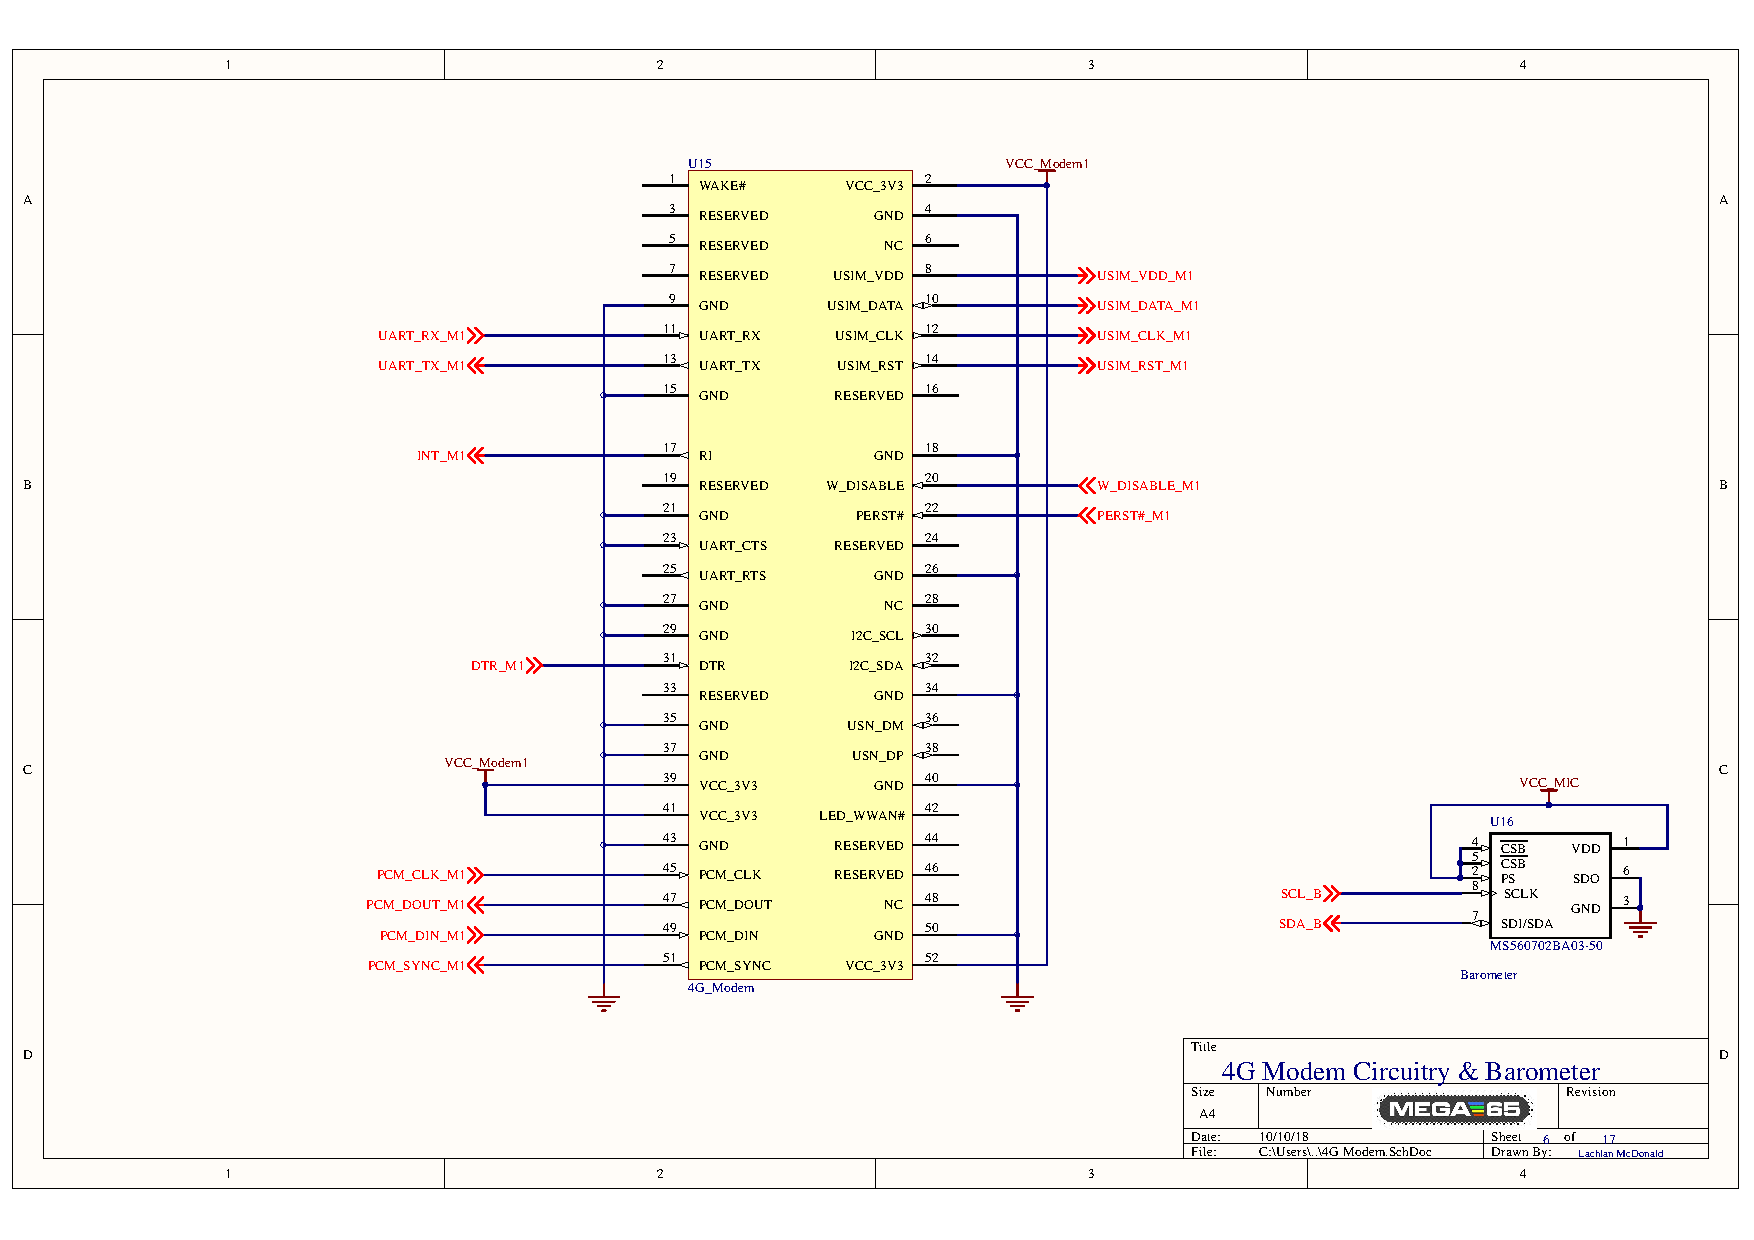
\includepdf[pages=-, angle=90]{MEGAphone.pdf}
%% Appendix Template

\chapter{PCB Layout} % Main appendix title

\label{AppendixB} % Change X to a consecutive letter; for referencing this appendix elsewhere, use \ref{AppendixX}

\includepdf[pages=-, angle=90]{Appendices/PCB_Final_Artwork.pdf}
%% Appendix Template

\chapter{Bill Of Materials} % Main appendix title

\label{AppendixC} % Change X to a consecutive letter; for referencing this appendix elsewhere, use \ref{AppendixX}

%\eject \pdfpageheight=40in
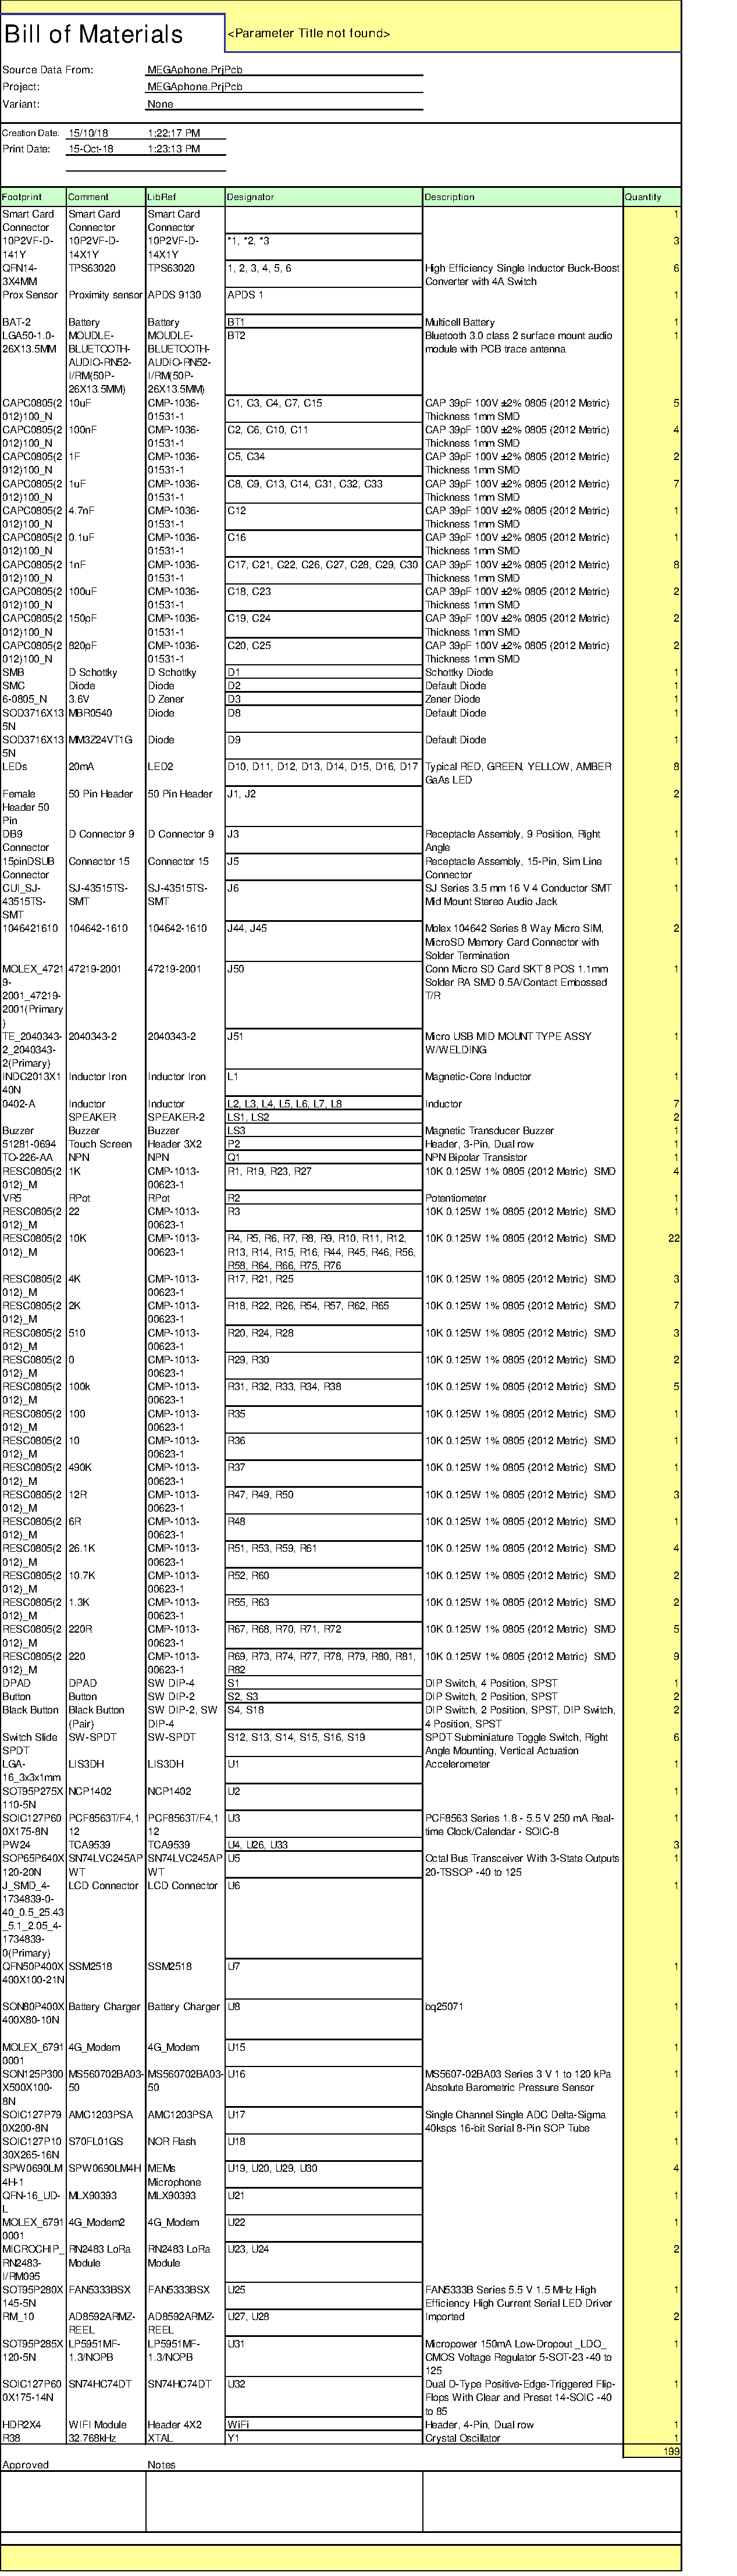
\includepdf[fitpaper=true, pages=-]{Appendices/BOM.pdf}

%\eject \pdfpageheight=297mm


%----------------------------------------------------------------------------------------
%	BIBLIOGRAPHY
%----------------------------------------------------------------------------------------
\bibliographystyle{ieeetr}
\bibliography{reference_library}

%----------------------------------------------------------------------------------------

\end{document}  
